\documentclass{UoYCSproject}

\usepackage[backend=biber]{biblatex}
\usepackage{graphicx}
\usepackage{float}
\usepackage{booktabs}
\usepackage{caption}
\usepackage{listings}
\usepackage{color}
\usepackage{amsmath}
\usepackage{algorithm}
\usepackage[noend]{algpseudocode}
\usepackage{xparse}
\usepackage{amssymb}
\usepackage{pdflscape}
\usepackage{longtable}
\usepackage{geometry}
\usepackage[toc,page]{appendix}
\usepackage{subcaption}
\usepackage{pdfpages}

\setcounter{secnumdepth}{4}

\newcommand{\ra}[1]{\renewcommand{\arraystretch}{#1}}
\renewcommand{\algorithmicrequire}{\textbf{Input:}}
\renewcommand{\algorithmicensure}{\textbf{Output:}}
\newcommand\tab[1][1cm]{\hspace*{#1}}
\NewDocumentCommand{\codeword}{v}{%
\texttt{{#1}}%
}

\addbibresource{references.bib}
\author{Sophie Wood}
\title{Model-driven software migration between microcontrollers}
\date{Version 0.1, 2018-May-16}
\supervisor{Simos Gerasimou}
\SWE
% TODO update wordcount
\wordcount{0}

% TODO update includes/excludes
\includes{Appendices TODO}

\excludes{TODO}

% TODO update abstract
\abstract{TODO}

% TODO update acknowledgements
\acknowledgements{TODO}

%TODO add statement of ethics

\begin{document}
\maketitle
\listoffigures
\listoftables

\chapter{Introduction}
\section{Background and Motivation}

Bartels et al. define obsolescence as ``materials, parts, devices, software, services and processes that become non-procurable from their original manufacturer or supplier'' \parencite{bartels2012strategies}. Both software and hardware can be subject to obsolescence problems. 

Issues with hardware obsolescence have been driven by the growth of the electronics industry. This has reduced the life cycle of electronic parts as competitors release products with better functionality and features. Existing products are no longer commercially viable and therefore go out of production \parencite{bartels2012strategies}. This is a particular issue in the defence/aerospace sectors as the typical life cycle of a system is 20-30 years or longer \parencite{rojo2010obsolescence}. As such, parts will become unavailable before the system is completed. Singh et al. found that these systems ``often encounter obsolescence problems before they are fielded and always during their support life'' \parencite{singh2006obsolescence}.

Obsolescence is also a concern in the software industry. Businesses must continuously update their products in order to stay ahead. Bill Gates has said: 
\begin{quote}
``The only big companies that succeed will be those that obsolete their own products before someone else does.'' \parencite{bartels2012strategies}
\end{quote}
There are three main causes of software obsolescence: \textit{logistical} -  digital media obsolescence, formatting or degradation terminates or limits access to software; \textit{functional} - hardware, requirements, or other software changes to the system obsolete the functionality of the software; and \textit{technological} - the sales and/or support for commercial off the shelf (COTS) software terminates \parencite{sandborn2007obsolescence}. 

In addition, software obsolescence can be driven by hardware obsolescence and vice versa. Another issue is lack of skills. For example, there may be a limited number of people that are competent in the language the system is written in. If these people leave the company, the system can no longer be maintained \parencite{rajagopal2014software}. 

Again avionics/military and other ``safety-critical'' systems particularly struggle with software obsolescence issues as even small changes may have to go through extensive and costly qualification/certification processes \parencite{singh2006obsolescence}. Consequently, software obsolescence costs can equal or exceed that of hardware \parencite{sandborn2007obsolescence}. Despite this, strategies for obsolescence mitigation/management have generally focused on hardware obsolescence problems. It is important that both hardware and software obsolescence issues are tackled as these problems can be incredibly costly to these industries. For example, the US Navy estimates that obsolescence problems can cost up to \$750 million annually \parencite{adams2005getting}. Sandborn and Myers also found that sustainment costs (which include costs related to obsolescence) dominate the system costs in the case of development of an F-16 military aircraft \parencite{sandborn2008designing}. 
 
Current strategies for mitigating software obsolescence issues are insufficient. Proactive measures (e.g. improving code portability or using open-source software) often require either a large amount of resources or resources that are unavailable. Reactive strategies for tackling obsolescence (e.g. software license downgrades, source code purchase or third party support) may not always be possible. When these methods are inadequate, the legacy system may have to be redeveloped or rehosted \parencite{sandborn2007obsolescence}. However, many such software modernisation projects are abandoned or not completed within the planned timescale/budget \parencite{kowalczyk2009model}. 

If redevelopment projects can be automated or even partially automated, they can more easily be completed on time. \parencite{gerasimou2017technical} uses code analysis and code-based transformations to partially automate the process of adapting software to work with different libraries as well as migrating software between hardware platforms. Although this approach is successful, the process may not scale well. For example, in one stage of the process of adapting code to use a new library, an abstraction layer is generated that has the same usage behaviour as the obsolete library. This is then used to replace the usages of the legacy library. If applied to a project with many library usages, this could generate a large amount of additional code in the modernised project which may make it difficult to maintain. 

An alternative approach is to use model-driven software modernisation (MDSM) for (partial) automation of modernisation projects. MDSM is based on the use of model-driven engineering (MDE) principles such as models and transformations to facilitate the migration process (MDE and its application to software modernisation are discussed in more detail in Sections \ref{mde_approaches} and \ref{mde_bg}). For example, model-to-model transformations can be used to map a model of the legacy code to a model of the new system. A model-to-text transformation can then be applied to this new model to generate code for the new version of the system.

MDSM is a promising approach as it has already been proved feasible in industry by the Sodifrance\footnote{https://www.sodifrance.fr/} company. For example, they were able to migrate a large-scale banking system (at a size of around one million lines of code) to J2EE \parencite{fleurey2007model}. Kowalczyk and Kwieci\'nska have also demonstrated the viability of MDSM by modernising a project written in Java 1.4 and the Hibernate 2.x framework into Java 1.5 and Hibernate 3.x \parencite{kowalczyk2009model}. One benefit of MDSM is that tools (e.g. model discoverers) can sometimes be reused between projects making subsequent modernisation projects quicker and cheaper to complete. For example, MoDisco is an open-source model-discoverer that can generate models from Java code \parencite{bruneliere2014modisco}.

The Defence Science and Technology Laboratory (DSTL) at the Ministry of Defence (MoD) have identified several instances of software obsolescence they would like to tackle. A problem of particular interest is ``the migration of an entire software system from a legacy hardware platform to a modern more powerful platform'' \parencite{gerasimou2017technical}. This report will explore how MDSM processes can be used to partially automate the migration of code between microprocessors. A case study implementing the migration of code between a Parallax Propeller Activity Board and an Arduino Uno will be used to demonstrate the approach developed.
 
\section{Project Goals}
TODO
\section{Project Scope}
TODO
\section{Report Structure}
TODO

\chapter{Literature Review}
The following chapter introduces the existing work on software obsolescence and the technical background required to understand this project. It begins with an overview of the existing approaches for software obsolescence mitigation in Section \ref{so_approaches} and in particular, MDE-based strategies in Section \ref{mde_approaches}. The specific problem of migration between microcontrollers and the existing methods for facilitating this are discussed in Section \ref{mc_migration} as well as how the MDSM-based method explored in this project is related. 

Sections \ref{mde_bg} and \ref{mc_bg} contain the technical background of the project including a brief overview of MDE and the chosen framework for this project as well as a description of the microcontrollers used for the case study.

\section{Existing Work}
\subsection{Approaches to Software Obsolescence} \label{so_approaches}
Rojo et al. identify some of the main methods of tackling obsolescence in their paper ``Obsolescence management for long-life contracts: state of the art and future trends'' \parencite{rojo2010obsolescence}. Although they identified many strategies for handling the obsolescence of electronic components, very few methods were relevant for dealing with software obsolescence.

The tools ``se-Fly Fisher'' and ``R2T2'' (Rapid Response Technology Trade) were identified as useful for managing software obsolescence. These tools are used for design refresh planning. Design refresh planning deals with obsolescence in a proactive manner by planning the best times for performing a redesign of the system during the sustainment stage of its lifecycle. 

Se-Fly Fisher uses the technology curves of each part of the system to: forecast how often a system baseline should change; identify replacement resources and estimate the benefit of each system baseline change \parencite{rojo2010obsolescence}.

Similarly, R2T2 can: forecast system obsolescence; allow for comparisons to alternative solutions; produce a life cycle obsolescence plan for the elements that require refreshment and plan when element replacements should occur \parencite{herald2009obsolescence}.

These forecasting tools may enable organisations to plan ahead and handle cases where equivalent parts/software are available. However, they cannot assist in the actual redesign or redevelopment process which can be time consuming and costly.

Similarly, Sandborn et al. identified very few approaches towards managing software obsolescence. The main methods they identified for mitigating software obsolescence were \parencite{sandborn2007obsolescence}:
\begin{description}
\item[(1) Software License Downgrade:] users can purchase licenses for the current product and apply them to older versions.
\item[(2) Source Code Purchase:] customers purchase the source code for the product.
\item[(3) Third Party Support:] a third party is contracted to maintain support for the software.
\end{description}
When possible, these approaches could reduce costs as the software does not have to be maintained in house or redeveloped. However, sometimes these methods may not be possible. Additionally, given that the system owners are so dependent on the legacy code, it puts them in a poor position for negotiating the prices for these contracts and so this approach could become costly.

\subsection{MDE Approaches to Software Obsolescence} \label{mde_approaches}
More recently, MDE approaches have been used to tackle software obsolescence problems where legacy code must be redeveloped. MDE allows some of the stages in migration to be automated, consequently reducing the timescale and costs involved.

The company Sodifrance has successfully been using MDE for development and migration projects for over ten years \parencite{fleurey2007model}. The general MDE approach to migration used by Sodifrance is shown in Figure \ref{fig:sodifrance_process}. The approach is separated into four stages as follow:

\begin{enumerate}
\item Firstly, the code of the legacy application is parsed in order to create a model of the legacy system. In Figure \ref{fig:sodifrance_process}, \textit{L} indicates the metamodel for the implementation language of the legacy code.
\item This model is then transformed to a Platform Independent Model (PIM) conforming to an ANT metamodel\footnote{An ANT metamodel contains packages to represent:
\begin{itemize}
\item Static data structures (close to the UML class diagram).
\item Actions and algorithms (it includes an imperative action language).
\item Graphical user interfaces and widgets.
\item Application navigation.
\end{itemize}}. This model represents a high-level view of the legacy code. This process is dependent on knowledge of the libraries and coding conventions used by the legacy platform.
\item Next the PIM has a model transformation applied to produce a Platform Specific Model (PSM) conforming to a UML metamodel. The high-level views from the PIM are adapted to fit the target platform.
\item Finally, code is generated from the PSM by using template-based text generation tools.
\end{enumerate}

\begin{figure}[h!]
  \centering
  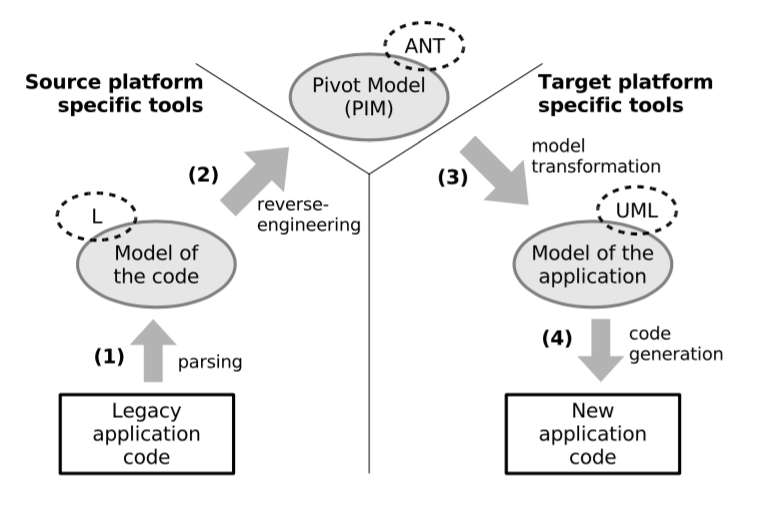
\includegraphics[width=0.6\linewidth]{graphics/sodifrance_mde.png}
  \caption{The general model-driven migration process used by Sodifrance \parencite{fleurey2007model}.}
  \label{fig:sodifrance_process}
\end{figure}

The first two steps of the process can usually be fully automated. However, the remaining stages need some manual effort. Tasks that could not be completed automatically are indicated in the generated code (e.g. by TODO directives in Java applications) and summarised into a task list in order to allow the manual process to be completed more efficiently.

Sodifrance demonstrated the effectiveness of their approach using a case study of migrating a large-scale banking system from Mainframe to J2EE.

Kowalczyk and Kwieci\'nska have also explored the use of MDE in software migration \parencite{kowalczyk2009model}. They identified two main approaches: the ``Reverse MDA approach'' (RMA) and the ``Direct Transformation Approach'' (DTA).

The RMA approach follows the same stages as that used by Sodifrance. The DTA approach shown in Figure \ref{fig:dta} reduces the number of stages involved in the transformation process by directly transforming between platform specific models. 

\begin{figure}[h!]
  \centering
  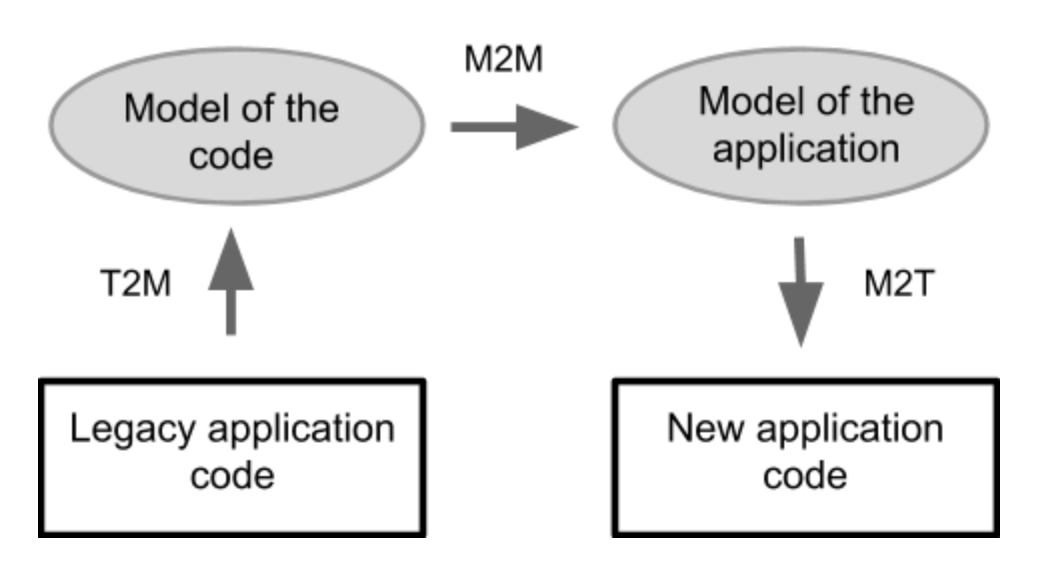
\includegraphics[width=0.6\linewidth]{graphics/dta.png}
  \caption{The stages involved in the ``Direct Transformation Approach''.}
  \label{fig:dta}
\end{figure}

The feasibility of both approaches was demonstrated by a case study migrating from Java 1.4 and the Hibernate 2.x framework to Java 1.5 and Hibernate 3.x. Based on qualitative analysis of the two approaches, they recommend to use an approach similar to DTA as it is often not the case that a transformation from the legacy code model to the PIM will exist. It is especially suited to cases where the code model and application model use the same metamodel. 

MDE approaches to software migration have many benefits. The primary reason is the ability to automate some of the stages in the migration process, consequently reducing the cost and time scale of projects. Secondly, parts of the process (e.g. model discoverers or transformations) can be reused between different migration projects which will again cut the cost of migration.

There are however, drawbacks to the MDE approach. There is a high cost of entry to start using MDE methods --- the initial development of processes and tools can be time consuming and expensive if open-source tools are not available. Secondly, a particular issue in commercial projects is that no code will be available until the initial analysis and tool development stage of the process is completed. In the case of the Sodifrance case study, code was not delivered until 10 months after the project had begun \parencite{fleurey2007model}. This can make customers nervous and reluctant to try this approach. On the other hand, once the initial stage is completed, the delivery rate of the code can be much faster than for a standard re-development approach.

One of the main considerations that must be made when choosing an MDE approach is the size of the project. If the project is small, it may be more expensive to use this method as the initial stages may take longer than manually migrating the code \parencite{fleurey2007model}. This is demonstrated in Figure \ref{fig:costvsize}.

\begin{figure}[h!]
  \centering
  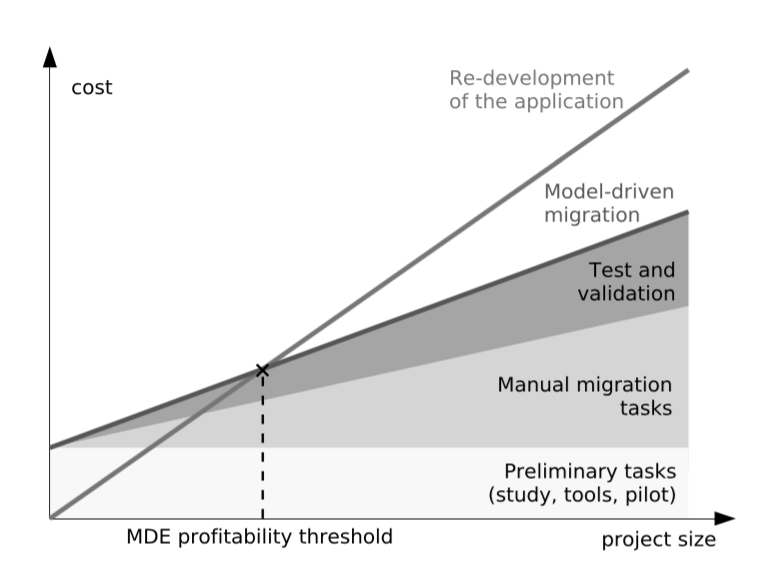
\includegraphics[width=0.6\linewidth]{graphics/costvsize.png}
  \caption{Project migration cost as a function of its size \parencite{fleurey2007model}.}
  \label{fig:costvsize}
\end{figure}

\subsection{Migration Between Microcontrollers} \label{mc_migration}
As mentioned previously, a particular problem of interest to the MoD is ``the migration of an entire software system from a legacy hardware platform to a modern more powerful platform'' \parencite{gerasimou2017technical}.

Atmel addressed the issue of migrating code between microcontrollers by reducing the learning curve for developers moving from development on 8-bit to 32-bit platforms. They aimed to achieve this by providing powerful debug facilities and development tools similar to established 8-bit development platforms \parencite{wilbrink2004facilitating}.

Although this strategy should reduce the migration effort, the code will still be have to be migrated manually which is error-prone and difficult. Additionally, the development of new tools adds extra overhead to the project, although these tools are reusable between projects.

Another approach for migrating code between microprocessors combines code analysis, code-based transformations and verification/validation techniques \parencite{gerasimou2017technical}. The procedure follows the following steps:
\begin{description}
\item[(1) Software system analysis (automated):] The source code and obsolete libraries are parsed to obtain abstract syntax trees (ASTs). The AST can be examined to indicate the elements using the obsolete library and help establish the system's dependency level.
\item[(2) Discovery of similar libraries (non-automated):] The development team identifies candidate libraries for replacement of the obsolete library.
\item[(3) Compatibility analysis of the discovered libraries (non-automated):] Candidate libraries are rejected if they don't conform to technical or semantic requirements.
\item[(4) Data visualisation (automated):] Used to analyse the software system and its coupling with the obsolete library.
\item[(5) Execute generation transformations (automated):] Firstly, an abstraction layer is generated that has the same usage behaviour as the obsolete library. Next the obsolete library usages are replaced with this abstract layer.
\item[(6) Mappings inference (non-automated):] A developer creates a list of mapping rules by inspection of the obsolete and replacement libraries.
\item[(7) Code population (non-automated):] A developer uses the mapping rules generated in stage 6 to populate the abstraction layer generated in stage 5.
\end{description}
This method was demonstrated to succeed in partially automating the migration of software between an Arduino and Raspberry Pi.

By automating some of the migration stages, the overall time and cost of software modernisation should be reduced. Another benefit is that the code analysis stages allow for potential risks to be detected early on. However, there is still a lot of manual effort required for migrating between libraries and in particular, generating mapping rules requires a developer with a strong understanding of both the new and obsolete libraries. Another issue is that adding the abstraction layer could lead to a large increase in the size of the code if the obsolete libraries are used frequently. This could make the code more difficult to maintain.

My project aims to explore an alternative approach for migrating code between microcontrollers by applying an MDE approach similar to that discussed in Section \ref{mde_approaches}. In doing so I aim to be able to (partially) automate the migration process, consequently reducing the time taken for migration whilst also avoiding issues associated with other methods such as code blow-up in \parencite{gerasimou2017technical}.

\section{Model Driven Engineering} \label{mde_bg}
Model Driven Engineering (MDE) was developed in order to address complexity within the problem space of computing. In the past, approaches for enabling programmers to develop code more easily have focused on simplifying the solution space. This was achieved by providing abstractions such as higher-level programming languages or providing operating systems to manage the difficulty of programming hardware directly. However, these solutions are unable to express domain concepts effectively, unlike MDE techniques \parencite{schmidt2006model}. Furthermore, it has been found that MDE can also be utilised in automating the software development process \parencite{bezivin2004search}.
\newline
The rest of this section introduces the terminology and main components of MDE as well as the MDE framework I will use in the project.

\subsection{Domain-Specific Modelling Languages (DSMLs)}
Meta-meta-modelling mechanisms such as the Object Management Group's (OMG) Meta Object Facility (MOF) can be used to create modelling languages for a given problem domain \parencite{mussbacher2014relevance}. The key components of the OMG's approach to DSMLs are \parencite{bezivin2001towards}:
\begin{description}
\item[Models:] A model is a simplification of a system built with an intended goal in mind. Models should be easier to use than the original system. This is achieved by abstracting out details of the system that are unnecessary for the target model's intended purpose.
\item[Meta-models:] A meta-model is the explicit specification of an abstraction (i.e. model). 
\item[Meta-meta-models:]  A meta-meta-model is used to define meta-models. In particular, the OMG define the MOF (Meta Object Facility) which is a self-defined meta-meta-model.
\end{description}

The relationships between these MDE concepts are summarised in Figure \ref{fig:metamodel_term}

\begin{figure}[h!]
  \centering
  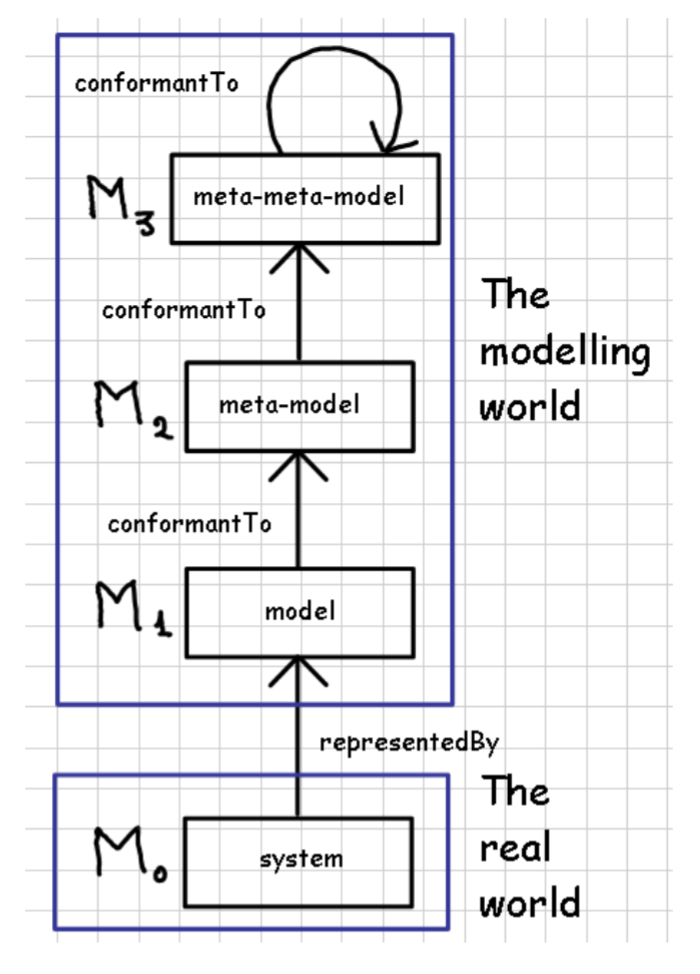
\includegraphics[width=0.5\linewidth]{graphics/metamodel_terminology.png}
  \caption{The relationship between the key concepts in MDE \parencite{bezivin2004search}.}
  \label{fig:metamodel_term}
\end{figure}


\subsection{Model Transformations}
There are three main categories of model transformation:
\begin{description}
\item[Model-to-model (M2M):] M2M transformations are used to translate source models to target models. The source and target models can be instances of the same or different meta-models \parencite{czarnecki2003classification}.
\item[Model-to-Text (M2T):] These can be considered a special case of M2M transformations. It is often the case that M2T transformations are used for code generation. The most common approach to M2T transformation is a template-based approach. A template contains mixtures of static text and dynamic sections that can be used to access information from the source model \parencite{czarnecki2003classification}.
\item[Text-to-Model (T2M):]  T2M transformations can be used to transform code to a model (conforming to a language meta-model). Model discoverer tools such as MoDisco \parencite{bruneliere2014modisco} are the easiest way to perform T2M transformations on code \parencite{kowalczyk2009model}.
\end{description}

\subsection{The Epsilon Framework}
% TODO may be worth comparing to M2T Xpand
Epsilon is a family of programming languages for model management tasks. It provides (among others) the following languages of interest \parencite{kolovos2010epsilon}:
\begin{description}
\item[Epsilon Object Language (EOL):] EOL is the common basis for the languages provided by Epsilon. It can be used for querying and modifying models.
\item[Epsilon Validation Language (EVL):] EVL is used for model validation.
\item[Epsilon Transformation Language (ETL):] ETL is used for M2M transformations.
\item[Epsilon Generation Language (EGL):] EGL is used for M2T transformations.
\end{description}
Epsilon also enables the use of ANT tasks to create workflows of different tasks (e.g. a validation followed by a
transformation followed by code generation) \parencite{kolovos2010epsilon}.
\newline
Epsilon has been chosen as the framework for this project over others for the following reasons:
\begin{itemize}
\item It is well documented with many tutorials as well as ``The Epsilon Book'' being freely available. Additionally, there is an active forum for any questions not answered by these sources \parencite{epsilonsite}.
\item It is well integrated with Eclipse (for example, syntax/error highlighting is provided in the editor and there are graphical tools for running/debugging programs) and has been an official project since 2006 \parencite{epsilonsite}.
\item Epsilon provides a connectivity layer (EMC). This layer allows EOL programs to access models of different modelling technologies including Eclipse Modelling Framework (EMF) models and XML documents \parencite{epsilonsite}.
\item I am already familiar with how to use the framework.
\end{itemize}

\section{Microcontroller Background} \label{mc_bg}
The project involves migration of code from a Parallax Propeller Activity Board to an Arduino Uno. However, since some features of the boards are different, this must be taken into account when migrating code. For example, the Propeller Activity Board has 16 digital pins whereas the Arduino Uno only has 14. In this case, code may need to be adapted to use different pins on the Arduino if it is migrated from the Propeller Activity Board. The following section highlights the important features and differences between the two boards as well as an overview of the board layout.

\subsection{Parallax Propeller Activity Board}
\begin{figure}[h!]
  \centering
  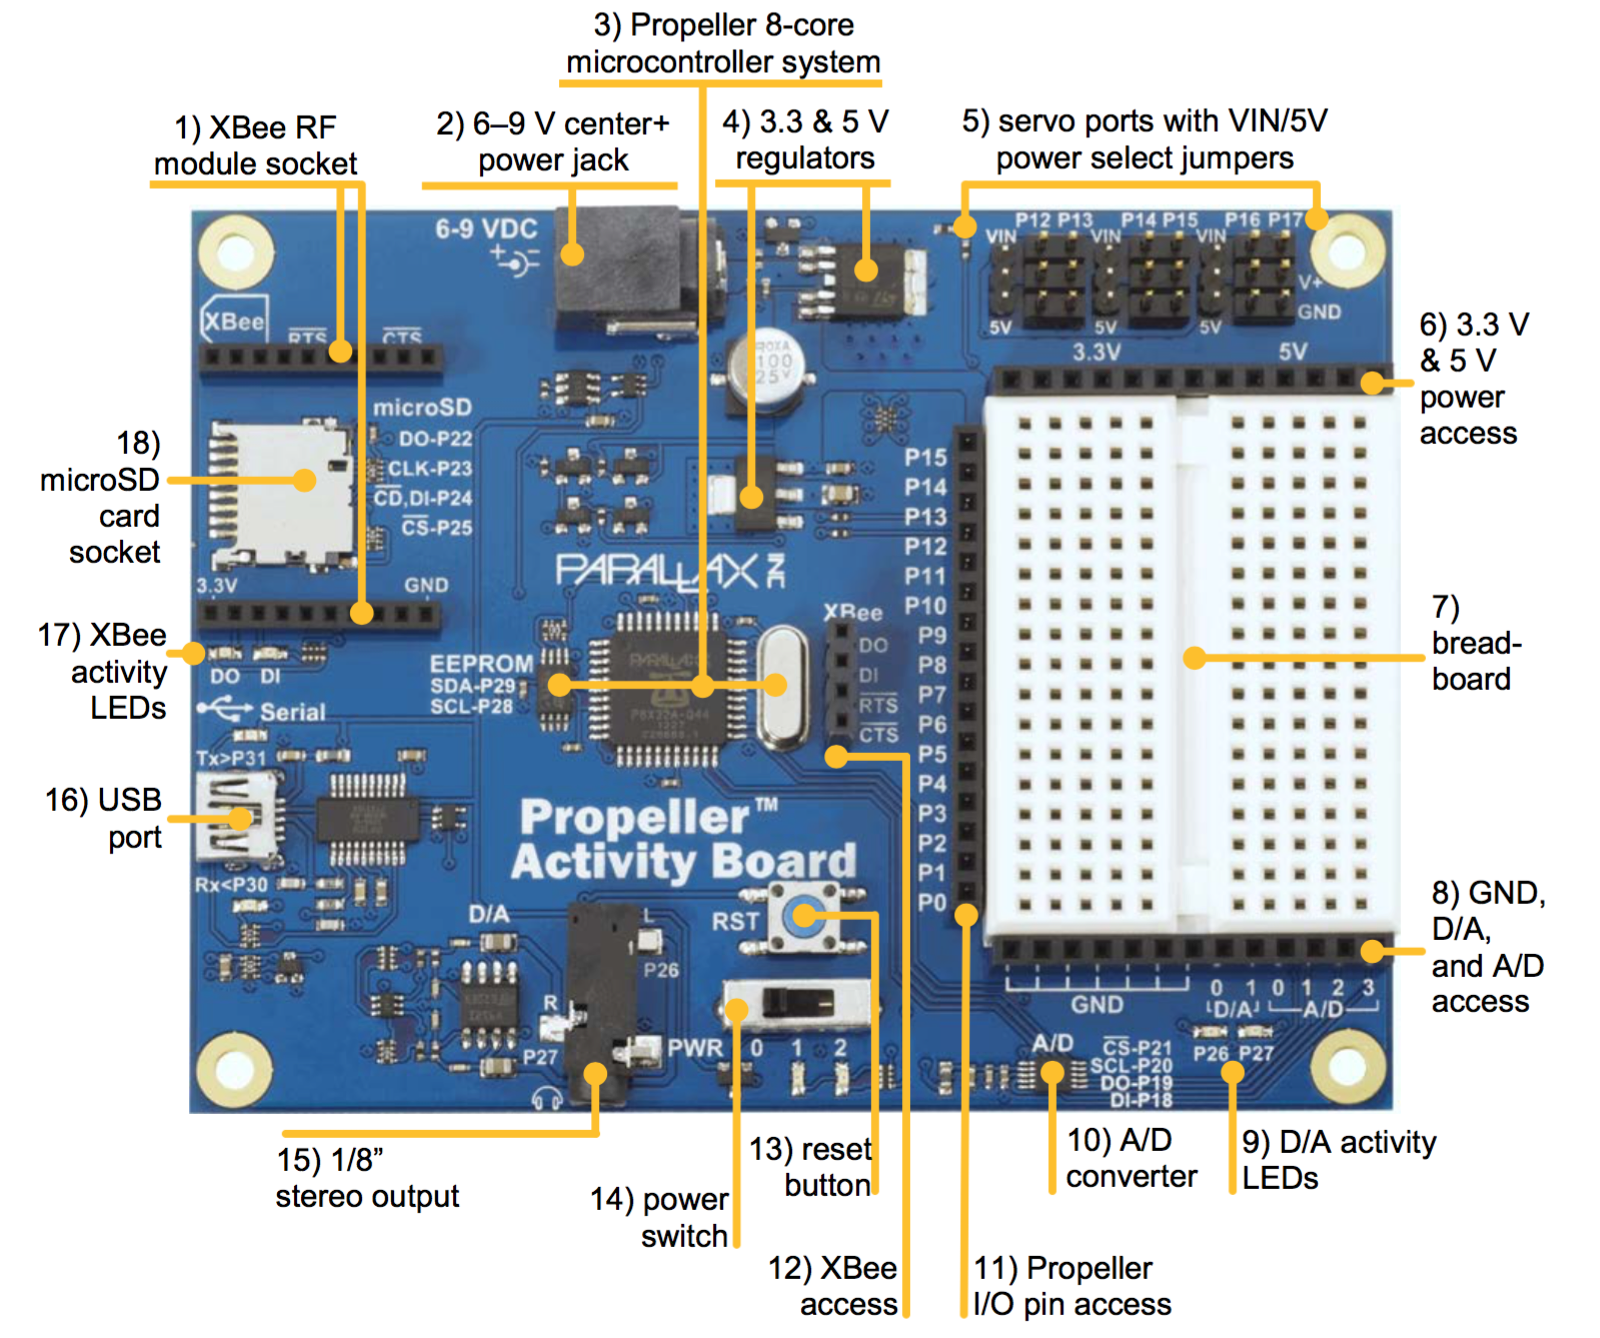
\includegraphics[width=0.6\linewidth]{graphics/propeller_board.png}
  \caption{Features of the Parallax Propeller Activity Board \parencite{propellerspec}.}
  \label{fig:prop_board}
\end{figure}

The key features of the Parallax Propeller Activity Board are \parencite{propellerspec}:
\begin{itemize}
\item Built-in 8-core Propeller P8X32A microcontroller
\item 64KB EEPROM
\item XBee wireless module socket
\item 16 digital I/O pins
\item 4 Analog-to-Digital pins
\item 2 Digital-to-Analog pins
\end{itemize}

\subsection{Arduino Uno}
%TODO: figure out which version I will be using
\begin{figure}[h!]
  \centering
  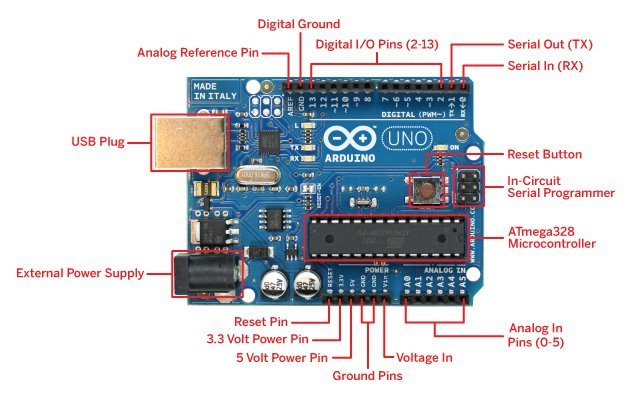
\includegraphics[width=0.8\linewidth]{graphics/arduino_board.jpg}
  \caption{Features of the Arduino Uno \parencite{arduinodiagram}.}
  \label{fig:arduino_uno}
\end{figure}

The key features of the Arduino Uno are \parencite{arduinospec}:
\begin{itemize}
\item Built-in single-core ATmega328 microcontroller
\item 32KB flash memory
\item 2KB SRAM
\item 1KB EEPROM
\item 14 digital I/O pins (6 provide PWM output)
\item 6 analog input pins
\end{itemize}

\chapter{Methodology}
This section summarises the methodology and tools used for managing this project. It begins with an overview of project management methodologies in Section \ref{overview_meth} and discusses the methodology chosen for this particular project in Section \ref{choice_meth}. Finally, the tools used for project management are discussed in Section \ref{proj_mgmt}.

\section{Overview of Methodologies} \label{overview_meth}
Project management methodologies can be roughly categorised as either traditional or agile methodologies. Each have their own strengths and weaknesses. Sections \ref{trad_meth} and \ref{agile_meth} provide an overview of these methodologies.
\subsection{Traditional Methodologies} \label{trad_meth}
Traditional approaches include the waterfall/linear methodology and the incremental strategy. The common features of these methodologies are that they are very structured and there is little room for deviation from the original plan. For example, the waterfall methodology splits the project into separate stages for software requirements gathering, systems requirements gathering, analysis, design, coding, testing and operations such that each section is completed before the next begins \parencite{royce1987managing}.

These strategies are best suited to projects that have a clear goal and clear solution. In this case, the use of these strategies can have many benefits. For example, the entire project is scheduled and resource requirements are known from the beginning. Additionally, this allows for team members to be distributed \parencite{fernandez2008agile}. However, heavy documentation is required and a detailed plan is needed from the start of the project. As such, it is difficult to adapt this pan to changes in requirements \parencite{fernandez2008agile}.

\subsection{Agile Methodologies} \label{agile_meth}
Agile methodologies are generally better at accommodating change than traditional methodologies as they repeatedly return to earlier stages in the development process. For example, Figure \ref{fig:agile_meths} shows a (simplified) view of the stages involved in the iterative, adaptive and extreme agile methodologies. Each approach goes through the full development process, tests and/or deploys the system (or a part of the system) and optionally returns to either the build, design or scope stage depending on the outcome of testing and deployment. This cycle can occur multiple times in the project lifecycle and is referred to as a sprint. Sprints generally last a few weeks but this can vary depending on the project.

\begin{figure}[h!]
  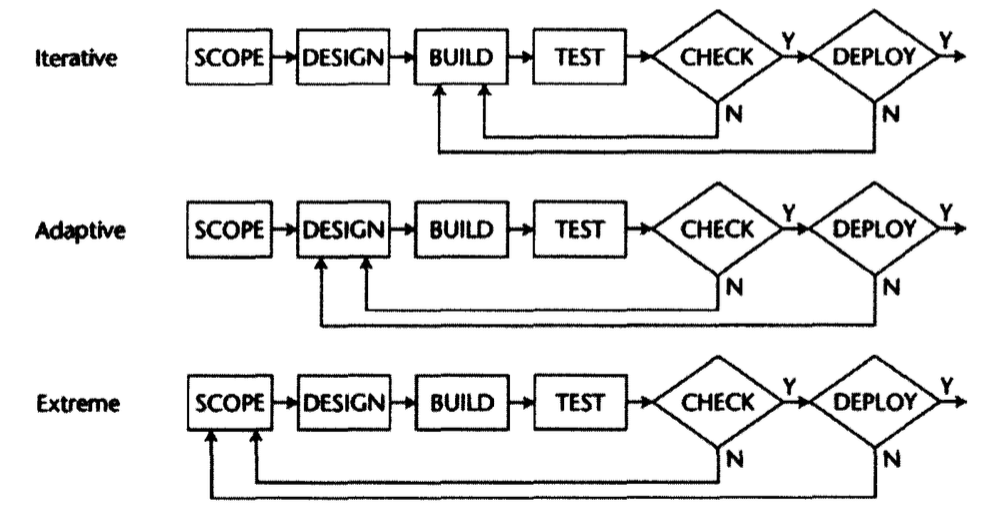
\includegraphics[width=\linewidth]{graphics/agile_methodologies.png}
  \caption{An overview of the iterative, adaptive and extreme agile methodologies \parencite{fernandez2008agile}.}
  \label{fig:agile_meths}
\end{figure}

As previously mentioned, the ability to return to earlier stages in the development process can help accommodate changing requirements. For example, the client can review what is produced at the end of each sprint and clarify or change requirements depending on the outcome. However, an agile approach requires much closer communication with the client which may not always be possible or desirable. Additionally, since requirements are not fixed for the duration of the project, the final product is not always clear from the start of the project \parencite{fernandez2008agile}.

\section{Choice of Methodology} \label{choice_meth}
The approach for this project is fairly well defined i.e. an MDE-based method will be used to perform software migration. However, the requirements are likely to change throughout the course of the project depending on the success of system prototypes. As such, the project is more suited to an agile methodology as this can more easily manage these changes. Additionally, I will be meeting with the project supervisor weekly which will allow us to work on updating the requirements as necessary and allows the project to be easily split into sprints beginning and ending at these meetings. In particular, the extreme methodology will be the most suitable as it allows for changing the scope which may be required if early research indicates the scope is unsuitable for the time allocated.

\section{Project Management} \label{proj_mgmt}
This section discusses the tools used in order to manage the project. This includes tools for task management as well as version control tools for the source code and report.

At the start of the project a GANTT chart was created in order to give a rough estimate for when certain parts of the project would be completed. This was not updated throughout the project and doesn't particularly fit with the agile methodology but it was helpful to ensure progress was being made at about the right pace. In particular, this was helpful for writing the report.

The GANTT chart was included in the project page which was created using Google Sites. This page was used to contain all the information for managing the project. In particular it was used for organising the literature review but also links to the task management tool for the project. Google Sites was chosen as it is free and can be easily adapted to suit the project. The literature review was organised by creating pages on the site for each category within the literature review (e.g. MDE background) and collecting notes from the relevant papers on these pages. The site also contained a list of papers to be read and a link to the Trello board for managing the writing and coding tasks. Trello is used as it is free and makes it easy to prioritise and organise tasks.

Git was used as the version control system for both the source code of the system and the documentation as it is free and I already had experience using it. The remote repositories were hosted on GitHub as it allows students to use private repositories for free. In particular, Git was chosen for managing the documentation over e.g. Google Drive as the report was written in \LaTeX~and so updates to the main report document could require changes to e.g. image files or the bibliography file. As such, it is easier to backup all these files at once using a single Git command rather than adding and deleting files from Google Drive. Additionally, the file history is saved using Git so it is easier to return to previous versions of the documentation.

\chapter{Requirements} \label{reqs}
This chapter discusses the requirements that must be satisfied in order to consider the project successful. Firstly, Section \ref{req_gathering} introduces the sources used to derive requirements including the relevant stakeholders for the project. Then Sections \ref{stakeholder_reqs} and \ref{sys_reqs} summarise the stakeholder and system requirements respectively. Each requirement is assigned an identifier and a priority based on the MoSCoW categorisation system \parencite{moscow}. In decreasing order, the priority levels each requirement can have are \textbf{M} (must have), \textbf{S} (should have), \textbf{C} (could have) and \textbf{W} (won't have).

\section{Requirements Elicitation} \label{req_gathering}
This section discusses the main sources considered for deriving requirements. Firstly, a summary of the initial project statement is presented in Section \ref{proj_stmt} as this is helpful for deriving the functional requirements for the project. Secondly, stakeholders for the project are identified in Section \ref{stakeholders} in order to enable gathering of stakeholder requirements.

\subsection{Project Statement} \label{proj_stmt}
The initial project statement is as follows: 
\begin{quote}
``This project aims to design and develop an extensible MDE-based infrastructure for migrating software applications between microprocessors. In particular, the project will enable:
\begin{itemize}
\item analysis and extraction of source code deployed on the old microprocessor
\item migration of extracted source code to the new microprocessor''
\end{itemize}
\end{quote}

\subsection{Stakeholders} \label{stakeholders}
Stakeholders are parties that are interested in the development of the project and therefore their goals must be taken into account when deriving requirements. The rest of this section introduces the roles of the primary stakeholders and gives a high-level overview of their objectives for the project.

\begin{description}
\item[Student/Project Developer:] Responsible for research, system design, development and testing. Primarily interested in demonstrating the efficacy of an MDE based approach to software migration and successfully completing the project on time.

\item[Project Supervisor:] Responsible for meeting regularly with the student and guiding the research for the project. Their goal is also for the system to be finished within schedule.

\item[Software Obsolescence Researchers:] Although not directly involved in the project, the results of the project may be of interest to researchers in the field of software obsolescence. In particular, the project explores an alternative approach to the migration of software between microcontrollers presented in \parencite{gerasimou2017technical}. This is a particular problem of interest to the DSTL. However, they are specifically investigating migration between their own microcontrollers such as the FS P4080. Therefore, they would require that the system is easily understandable and can be adapted to work with microcontrollers other than the Parallax Propeller Activity Board and the Arduino Uno.

\item[End Users:] No end users are directly involved in the project. However, some people may want to use the resulting system as is to migrate software from a Parallax Propeller Activity Board to an Arduino Uno. In this case, their main priority would be usability of the system. Additionally, it is important that the performance of the migrated software is not significantly worse than the source application. However, as this is a very specific scenario, it is unlikely that this user group will be very large. Similarly to software obsolescence researchers, it may be more useful to end users if the system can be easily modified to support migration between microcontrollers other than the Parallax Propeller Activity Board and Arduino Uno.
\end{description}

\section{Stakeholder Requirements} \label{stakeholder_reqs}
Table \ref{table:stakeholder_req} summarises the stakeholder requirements for the system. Each requirement has an identifier of the form S-X (where X is an integer).
\begin{table*}[h!]\centering
\ra{1.3}
  \begin{tabular}{@{}p{0.1\textwidth}p{0.15\textwidth}p{0.75\textwidth}@{}} \toprule 
  \textbf{ID} & \textbf{Priority} & \textbf{Description} \\
  \midrule
  S-1 & M & Users can provide the system with the source code for a Parallax Propeller Activity Board and target code for the Arduino Uno will be generated. \\ 
  S-2 & M & Users can easily adapt the system to support migration of software between different microprocessors. \\
  S-3 & S & Users can easily determine sources of errors when using the system. \\
  S-4 & S & Users can easily identify areas of the target code that cannot automatically be migrated and must be manually completed. \\
  S-5 & S & The performance of the migrated code is not significantly worse than the source application. \\
  \bottomrule
  \end{tabular}
\caption{Stakeholder Requirements}
\label{table:stakeholder_req}
\end{table*}

\section{System Requirements} \label{sys_reqs}
The following section summarises the functional and non-functional requirements of the system. Each functional requirement is assigned an identifier of the form F-X (where X is an integer) and each non-functional requirement is assigned an identifier of the form NF-X (where X is an integer).

Note that valid source code refers to an application which compiles and runs correctly on the source microprocessor and only uses hardware capabilities provided by both microcontrollers.
\newpage
\subsection{Functional Requirements}
Table \ref{table:func_req} summarises the functional requirements and their acceptance criteria for the system.
\begin{table*}[h!]\centering
\ra{1.3}
  \begin{tabular}{@{}p{0.05\textwidth}p{0.1\textwidth}p{0.425\textwidth}p{0.425\textwidth}@{}} \toprule 
  \textbf{ID} & \textbf{Priority} & \textbf{Description} & \textbf{Acceptance Criteria} \\
  \midrule
  F-1 & M & The target microcontoller running the migrated code (potentially with manual additions) displays the same behaviour as the source microcontroller, provided the source code is valid. & Manual inspection of the migrated application confirms the behaviour is the same as the source application. \\
  F-2 & M & The migrated code deploys without errors on the target microcontroller if the provided source code is valid. & Manual inspection of the migration process confirms a valid source application can be migrated without errors. \\
  F-3 & S & The system displays appropriate errors when the source code cannot be migrated (e.g. there are errors in the source code or hardware incompatibilities). & Errors are thrown when invalid source code is provided to the migration process. \\  
  F-4 & S & The system clearly indicates any errors that have occurred during its use (e.g. the migration process fails). & Errors are thrown if the migration process fails. The errors clearly indicate the source of the problem. \\
  F-5 & S & The system should indicate any parts of the code that must be manually completed. & Manual inspection of the migrated code confirms that all parts of the code that must be manually completed are clearly indicated (e.g. by TODO directives). \\
  \bottomrule
  \end{tabular}
\caption{Functional Requirements}
\label{table:func_req}
\end{table*}

\subsection{Non-Functional Requirements}
Table \ref{table:non_func_req} summarises the non-functional requirements and their acceptance criteria for the system.
\begin{table*}[h!]\centering
\ra{1.3}
  \begin{tabular}{@{}p{0.08\textwidth}p{0.1\textwidth}p{0.41\textwidth}p{0.41\textwidth}@{}} \toprule 
  \textbf{ID} & \textbf{Priority} & \textbf{Description} & \textbf{Acceptance Criteria} \\
  \midrule
  NF-1 & M & The system should be easy to adapt to support migration between different microcontrollers. & Manual inspection of the system should indicate that it is easy to adapt. For example, if the system is based on an established MDE framework it will be easier to adapt as there will be more documentation available. \\
  NF-2 & S & The system should display a high-level of encapsulation. & Manual inspection of the system should indicate measures have been taken to facilitate encapsulation. For example, separation of hardware-dependent parts of the code. \\
  NF-3 & S & The migrated code should not be significantly larger than the source code. & Migrated code is of a size acceptable to the stakeholder. \\
  NF-4 & S & The migrated code should exhibit similar performance to the source code. & Migrated code runs in a duration acceptable for the stakeholder. \\
  
  \bottomrule
  \end{tabular}
\caption{Non-Functional Requirements}
\label{table:non_func_req}
\end{table*}

\newpage
\section{Requirements Traceability Matrix}
The requirements traceability matrix shown in Table \ref{table:traceability} shows how stakeholder requirements correspond to system requirements.
\begin{table*}[h!]\centering
\ra{1.3}
  \begin{tabular}{@{}p{0.4\textwidth}p{0.4\textwidth}@{}} \toprule 
  \textbf{Stakeholder Requirements} & \textbf{System Requirements} \\
  \midrule
  S-1 & F-1, F-2 \\
  S-2 & NF-1, NF-2, NF-3 \\
  S-3 & F-2, F-3, F-4 \\
  S-4 & F-5 \\
  S-5 & NF-4 \\
  \bottomrule
  \end{tabular}
\caption{Requirements Traceability Matrix}
\label{table:traceability}
\end{table*}

\chapter{Design and Implementation}
This chapter of the report discusses the decisions made in designing and implementing the system for supporting the migration of software from a Parallax Propeller Activity Board to an Arduino (these will be referred to as the source and target respectively). The system is implemented as an Eclipse plugin to assist in usability. Firstly, the high-level architecture of the plugin will be presented in Section \ref{high_lev_arch} along with the design rationale. This will be followed by an examination of the low-level architecture and implementation of these components in Sections \ref{fritz_design} to \ref{parallax_design}.


\section{High-Level Architecture} \label{high_lev_arch}
\begin{figure}[h!]
  \centering
  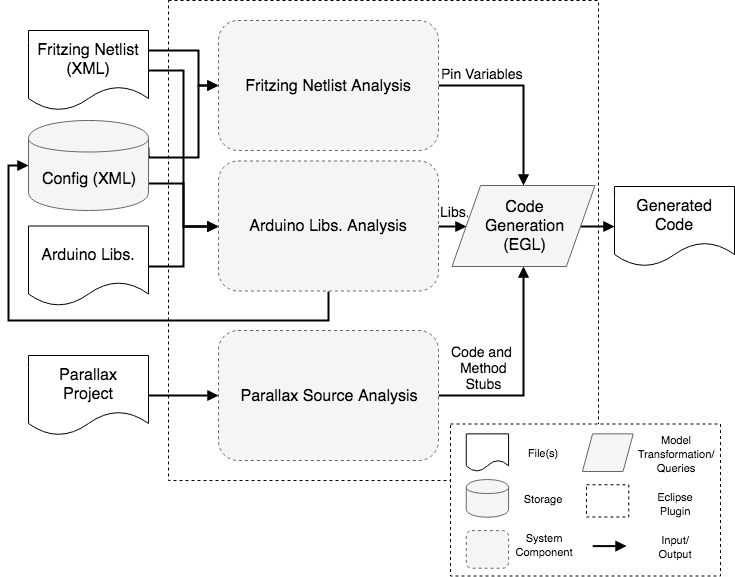
\includegraphics[width=0.8\linewidth]{graphics/high_level_overview.png}
  \caption{A high-level overview of the system.}
  \label{fig:high_level_overview}
\end{figure}

\subsection{Overview}
Figure \ref{fig:high_level_overview} shows the high-level architecture of the system. There are three main components to the system: Fritzing netlist analysis, Arduino libraries analysis and Parallax source code analysis. Each of these components produces information that contributes to code generation. The code generation is coordinated by an EGL transformation that takes the data from these components and generates a C file as output. This file acts as a basis for code that is compatible with the target platform. 

\begin{figure}[h!]
  \centering
  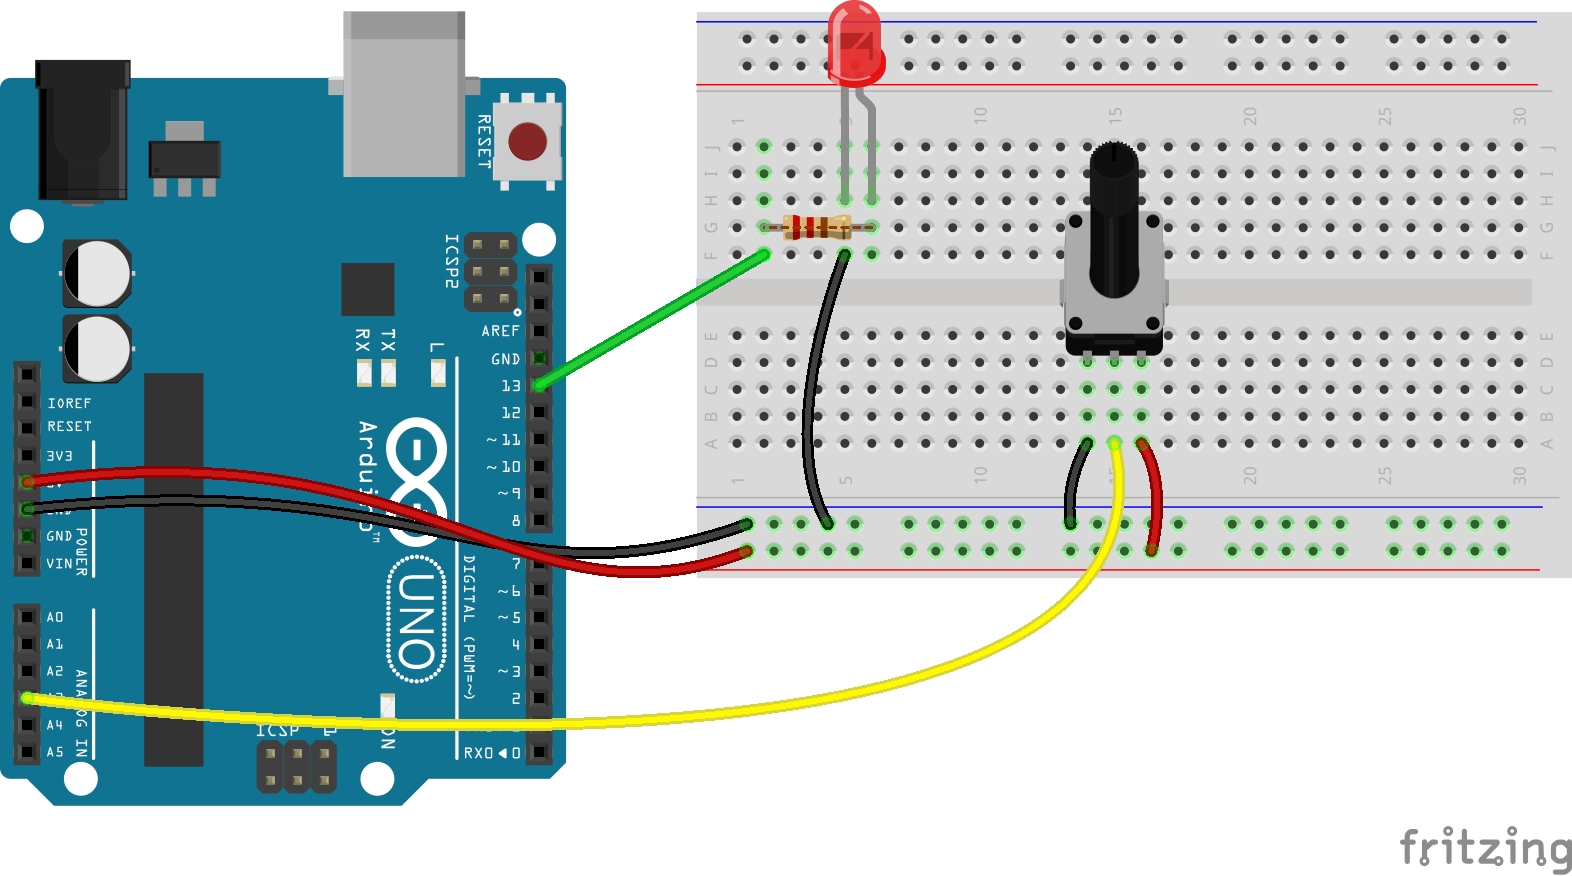
\includegraphics[width=0.6\linewidth]{graphics/fritzing_graphic.png}
  \captionof{figure}{An example Fritzing diagram.}
  \label{fig:fritz_graph}
\end{figure}

Fritzing\footnote{http://fritzing.org/home/} is open-source software that (among other uses) enables the user to create circuit diagrams and export a netlist\footnote{An XML file encapsulating all the parts and connections in the circuit}. Figures \ref{fig:fritz_graph} and \ref{fig:fritz_net} show a Fritzing diagram and part of a netlist for that diagram. The goal of the Fritzing netlist analysis component is to make it simpler to handle cases where the source and target platform have different pin configurations for a functionally equivalent circuit. For example, an LED may be attached to pin 12 on the source board and pin 6 on the target. Manually changing the references to this pin number can be error prone. Given a Fritzing netlist and a config file (containing additional information about Fritzing parts) this component calculates which pin of the board each part is connected to. This information is passed to the Code Generation EGL transform and used to generate pin variables in the output file.

\begin{figure}[h!]
  \centering
  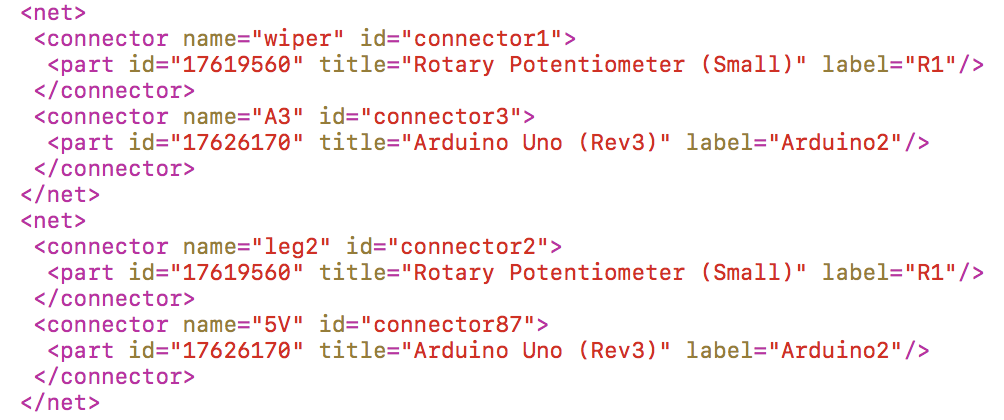
\includegraphics[width=0.8\linewidth]{graphics/fritzing_netlist.png}
  \captionof{figure}{Part of the netlist generated for Figure \ref{fig:fritz_graph}.}
  \label{fig:fritz_net}
\end{figure}

The goal of the Arduino libraries analysis component is to aid in mapping between source and target platform libraries. This is acheived by suggesting to the user suitable target platform libraries for the parts in the Fritzing netlist. Analysis is performed based on these parts and the Arduino header files to propose suitable libraries. Additionally, chosen libraries are recorded in the config. file and this is used to inform the suggestions when the system is run subsequently. The libraries chosen by the user are passed to the Code Generation EGL transform and used to add suitable include statements to the output file.

Finally, the goal of the Parallax source analysis component is to take the code for the source platform and modify it to make it suitable for the target platform and indicate any areas of the code that need manual modification. Source-platform-dependent constructs are identified during the analysis and this information is passed to the Code Generation EGL transform. Code that does not need modification is passed as is. For example, the method signatures of source platform library function calls are identified in the analysis. These signatures are then used to generate empty method stubs in the output file with TODO directives indicating these need to be manually replaced.

\subsection{Design Rationale}
Based on the requirements and stakeholders outlined in Chapter \ref{reqs}, reusability and modifiability were identified as the key quality attributes for the system. Based on the potential usage of Software Obsolescence Researchers, it is important that the system exhibits reusability so that successful components of the system are able to be used easily within other projects. As such, the system was designed to have loose coupling between components, in particular the three main components shown in Figure \ref{fig:high_level_overview}. This diagram clearly shows each of these elements works independently of the others and so could easily be reused. 

It is also crucial that the system displays a high degree of modifiability to support requirement S-2: ``\textit{Users can easily adapt the system to support migration of software between different microprocessors.}''. This is again supported by loose coupling between components. Another decision to support modifiability was to use a configuration file as input to the components analysing the Fritzing netlist and Arduino libraries. This file contains information that could have been hardcoded into each component. However, using a configuration file allows this to be easily replaced for supporting migration between different platforms.

\section{Fritzing Netlist Analysis} \label{fritz_design}
\begin{figure}[h!]
  \centering
  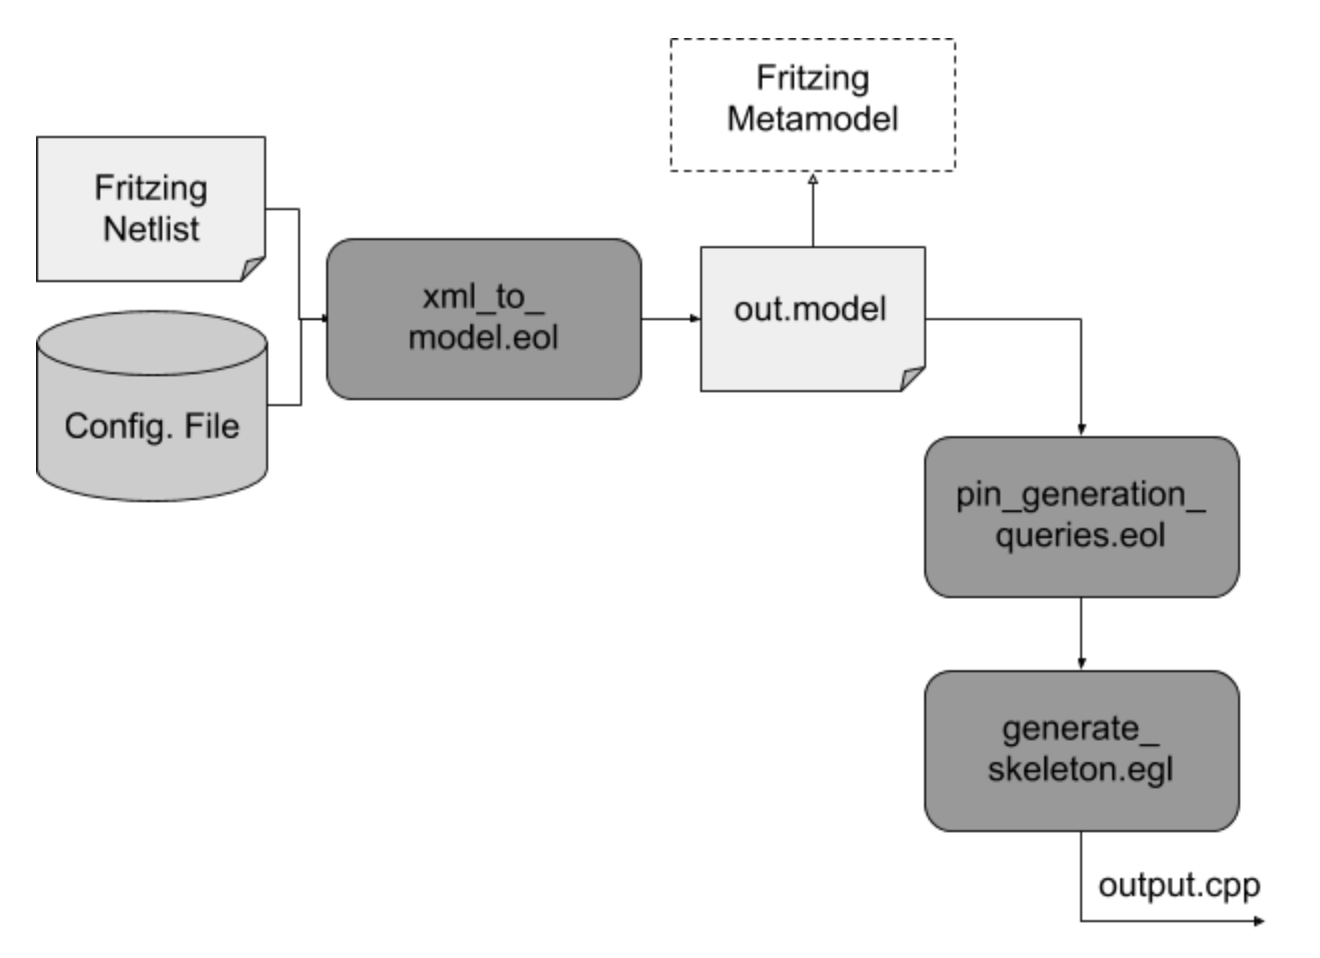
\includegraphics[width=0.8\linewidth]{graphics/fritzing_analysis.png}
  \caption{A more detailed view of the Fritzing netlist analysis component of the system.}
  \label{fig:fritzing_analysis}
\end{figure}

\subsection{Design}
The Fritzing netlist analysis component first consists of an XML to model transformation to extract the key information from the netlist. EOL queries are applied to this model to extract the connections from the parts to the target board. The Code Generation transform uses these queries in generating the pin variables for the output.

Although the netlist could be queried directly, the resulting model contains the information in a format making the queries easier to write as well as combining information from the config. file. This adds extra processing time but makes the code easier to understand which is more important given the requirements for the system.

Similarly, the output model from the transform could have been queried directly from the Code Generation EGL transform rather than having a separate EOL file to perform the queries. However, separating out the queries makes the logic in the EGL transform simpler as well as helping decouple the code generation from the implementation of the model/query logic. This improves the modifiability and reusability of this component.

\subsection{Implementation}

\begin{figure}[h!]
  \centering
  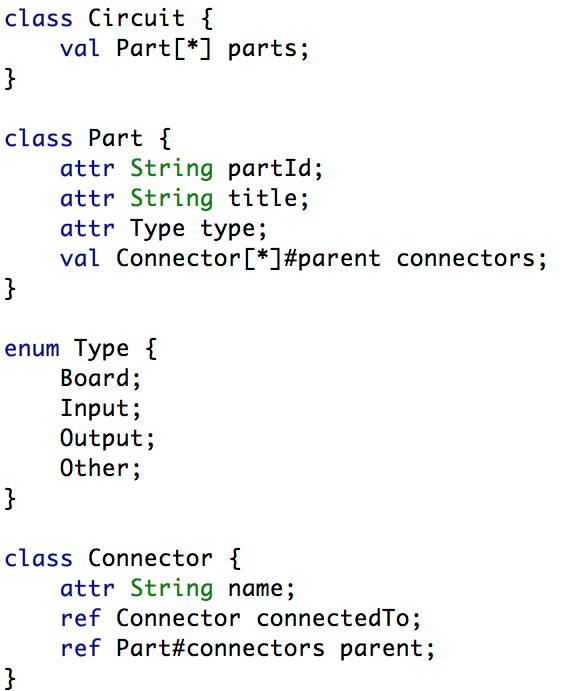
\includegraphics[width=0.4\linewidth]{graphics/fritz_metamodel.png}
  \caption{The EMF representation of the Fritzing metamodel.}
  \label{fig:fritz_metamodel}
\end{figure}

\subsubsection{Model Transform and Metamodel Design}
Figure \ref{fig:fritz_metamodel} shows the format for the Fritzing metamodel shown in Figure \ref{fig:fritzing_analysis}. The metamodel captures the essential information required to resolve the connections from parts to the Arduino board. Models conforming to this metamodel represent the circuit as a graph where nodes are parts and edges represent connections between the connectors of these parts. A graphical example of a model for the circuit in Figure \ref{fig:fritz_graph} is shown in Figure \ref{fig:fritz_model}.

\begin{figure}[h!]
  \centering
  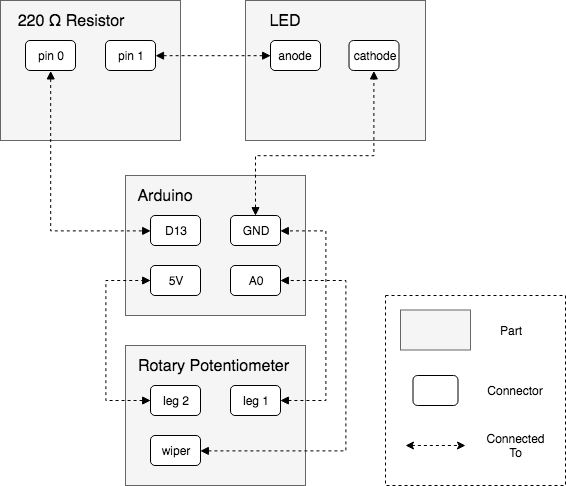
\includegraphics[width=0.6\linewidth]{graphics/fritz_model.png}
  \caption{A graphical representation of the model conforming to the metamodel shown in Figure \ref{fig:fritz_metamodel} for the circuit shown in Figure \ref{fig:fritz_graph}.}
  \label{fig:fritz_model}
\end{figure}

Most of the information for instantiating these models is extracted directly from the netlist. However, additional information about the type of parts is required. For example, when creating the pin variables in the output, we only want to generate values for devices read/written by the Arduino such as LEDs or potentiometers. Other parts, such as resistors, should not have pin variables generated. The config file (an example can be seen in Figure \ref{fig:config}) contains mappings between Fritzing part names and the type of the part. The part type is used to indicate whether or not variables should be generated for this component in the output file. This type information is stored as an attribute of the Part class in the model and is taken into account by the queries used to generate pin variables.

\begin{figure}[h!]
  \centering
  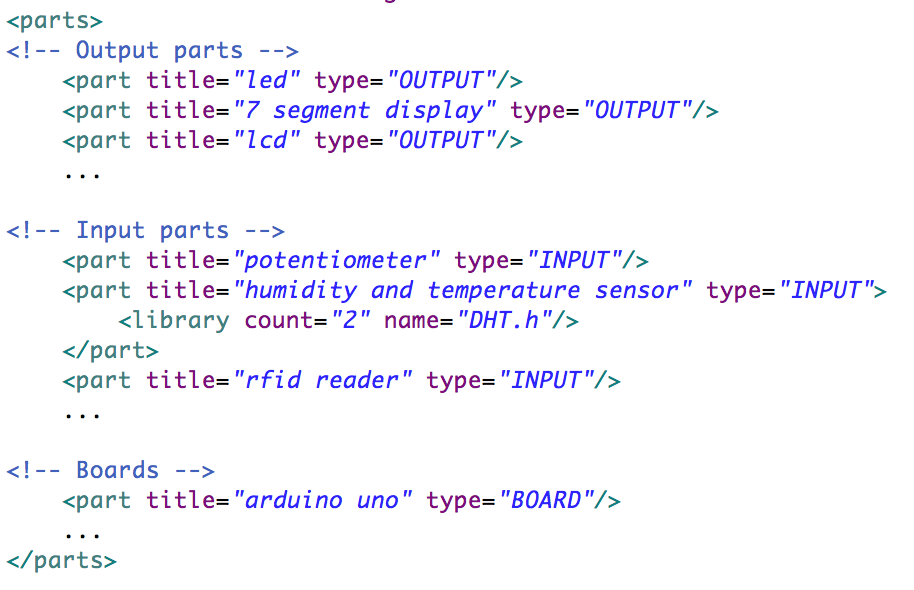
\includegraphics[width=0.6\linewidth]{graphics/config_file.png}
  \caption{Structure of the config file.}
  \label{fig:config}
\end{figure}

\subsubsection{Pin Generation Queries}
To find out which pins of the board parts in the circuit are connected to, a modified breadth-first search is performed on the Fritzing model. For each of the I/O connectors on the board, the connections in the model are followed until an input/output part is found. For example, resolving the connection to digital pin 13 (D13) in Figure \ref{fig:fritz_model} follows the connection to pin 0 of the 220$\Omega$ resistor, sees that this not an input/output part so follows the outgoing connections from this component (i.e. pin 1) to the anode of the LED. As this is a part tagged as an output type, a variable is then generated associating the LED with pin 13 on the Arduino board. The pseudocode below demonstrates the algorithm used for resolving the connections from the board to the input/output parts.

\begin{algorithm}
\caption{Calculate mapping from each pin on the board to its connected sensor(s)}
\begin{algorithmic}[1]
\Procedure{resolveBoardConnections}{$board$}
\For{$connector$ in $board.connectors$} 
\State $connectedSensor \leftarrow bfsResolveConnections(connector)$
\State $connections.put(connector, connectedSensor)$
\EndFor
\Return $connections$
\\
\EndProcedure
\end{algorithmic}
\end{algorithm}

\begin{algorithm}
\caption{Calculate set of connectors connected to $start$}
\begin{algorithmic}[1]
\Procedure{bfsResolveConnections}{$start$}
\State $queue.add(start)$
\While{\textbf{not} $queue.isEmpty()$}
	\State{$con \leftarrow queue.removeFirst()$}
	\If{\textbf{not} $visited.includes(con)$}
		\State {$visited.add(con)$}
		\State {$type \leftarrow con.parent.type$}

		\If{$type == INPUT$ \textbf{or} $type == OUTPUT$}
		\State{$connectors.add(con)$}
		\Else
			\State{$queue.add(con.connectedTo)$}
			\If{\textbf{not} $type == BOARD$}
				\For{$c$ in $con.parent.connectors$}
					\State{$queue.add(c)$}
				\EndFor
			\EndIf
		\EndIf
	\EndIf
\EndWhile
\EndProcedure
\end{algorithmic}
\end{algorithm}
% TODO: test assumption about only one component to each pin/ -> edit caption on first algorithm

\section{Arduino Library Analysis}
\begin{figure}[h!]
  \centering
  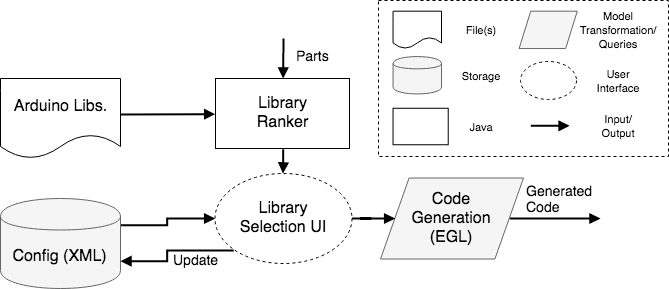
\includegraphics[width=0.8\linewidth]{graphics/arduino_library_analysis.png}
  \caption{A more detailed view of the Arduino library analysis component of the system.}
  \label{fig:arduino_analysis}
\end{figure}

\subsection{Design}
The Arduino Library Analysis component is used to suggest target platform libraries for each part in the Fritzing netlist. There are two methods used for library suggestion:
\begin{description}
\item[Library Ranker:] For each part, the Library Ranker component calculates a ranking for the suitability of each Arduino library (discussed in more detail in Section \ref{lib_ranker}).
\item[Config:] The config. file stores information about the previously used libraries for a given part. Whenever a library is chosen for a given part, the config file is updated with this choice. 
\end{description}

The Library Selection UI combines the library suggestions and displays them to the user. Once the choices have been made, it also coordinates the update of the config file and passes on the library choices to the Code Generation EGL transform. As the only information passed to the Code Generation transform is a list of libraries, there is no separate EOL file used in this component unlike in the Fritzing netlist analysis component (e.g. the Pin Gen. Queries in Figure \ref{fig:fritzing_analysis}).

As these library suggestion sub-components are logically independent, they have been separated to improve modifiability and reusability. Furthermore, the use of the config handler between the library selection UI and the config file abstracts away from the format of this file. This makes it easier to modify this subcomponent. For example, changing the format of the config file will not require a change in the library selection UI.

The config file is shared with the Fritzing Netlist analysis component of the system. Although this increases coupling between the components, it prevents duplication of information and therefore seemed suitable in this case.

\subsection{Implementation}

\begin{figure}[h!]
  \centering
  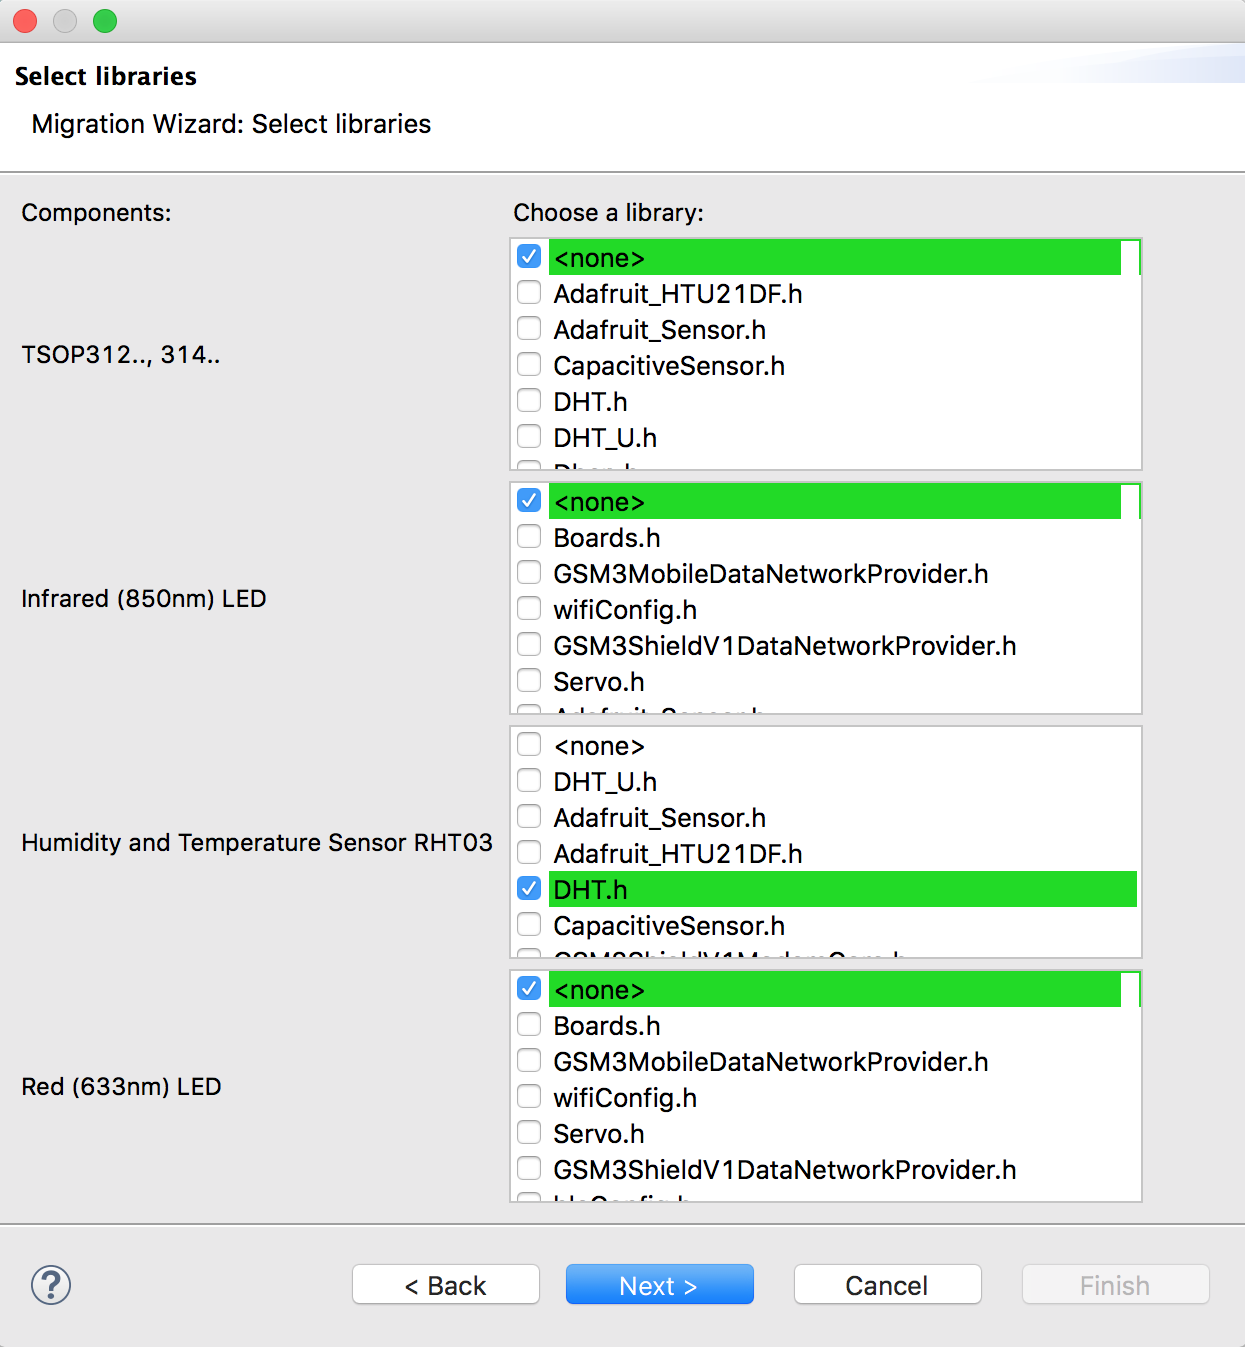
\includegraphics[width=0.8\linewidth]{graphics/lib_selection_ui.png}
  \caption{How the library suggestions are displayed to the user.}
  \label{fig:lib_selection_ui}
\end{figure}

Figure \ref{fig:lib_selection_ui} demonstrates how the library suggestions are displayed to the user. For each part in the netlist, a scrollable checklist allows users to select the appropriate library. The libraries are displayed based on the ranking provided by the Library Ranker component. The highlighted libraries are those that have previously been chosen for that part (as recorded by the config file).

\subsubsection{Library Ranker} \label{lib_ranker}
Given a part name and the Arduino library header files, the Library Ranker component calculates a ranking for the suitability of each library. The ranking is treated as an information retrieval task based on the part name. In other words, the Arduino libraries' header files are ranked based on similarity to the part's name. This makes the assumption that the most suitable library for a part will make some reference or include similar terms to the part's name. Although this is not intended to be an exact recommendation, it provides a useful heuristic for library suggestion.

For each library, the term frequency-inverse document frequency (\textbf{TFIDF}) value is calculated based on the part name. 

\textbf{TFIDF} is defined as:
\begin{equation}
w_{t,d} = \big(1 + log(tf_{f,d})\big) \times log\bigg(\frac{N}{df_t}\bigg)
\end{equation}

where:\\
\tab$df_t$ is the number of documents term $t$ occurs in\\
\tab$N$ is the number of documents in the collection\\
\tab$tf_{t,d}$ is the number of occurrences of term $t$ in document $d$\\
\\
In this case a document corresponds to a header file and a term corresponds to a word in the part name. The total ranking for a library is calculated by summing the \textbf{TFIDF} score for each term in the part name.
\textbf{TFIDF} was chosen as the ranking metric as it takes into account both the frequency of occurrence of a term in the library as well as its ``informativeness''. That is, a term is more informative if it appears in fewer documents of the collection (``informativeness'' effectively corresponds to the $log\Big(\frac{N}{df_t}\Big)$ term in the \textbf{TFIDF} equation). For example, if we consider the part \textit{humidity and temperature sensor} the term \textit{sensor} is less informative than \textit{humidity} as many parts have the term \textit{sensor} in the title and so will many header files. If we don't take the ``informativeness'' into account, any part that contains \textit{sensor} in the title is likely to rank highest the header file with the most occurrences of \textit{sensor} in the text, regardless of the type of sensor. Since \textit{humidity} is a less common term, using the \textbf{TFIDF} ranking will instead rank header files containing the less frequently occurring term \textit{humidity} higher.

\subsubsection{Config}
The config file stores the name of libraries chosen for each part as well as the number of times it has been chosen. For example, Figure \ref{fig:config} shows that the library "DHT.h" has been chosen twice for the humidity and temperature sensor.

\section{Parallax Project Analysis} \label{parallax_design}
\begin{figure}[h!]
  \centering
  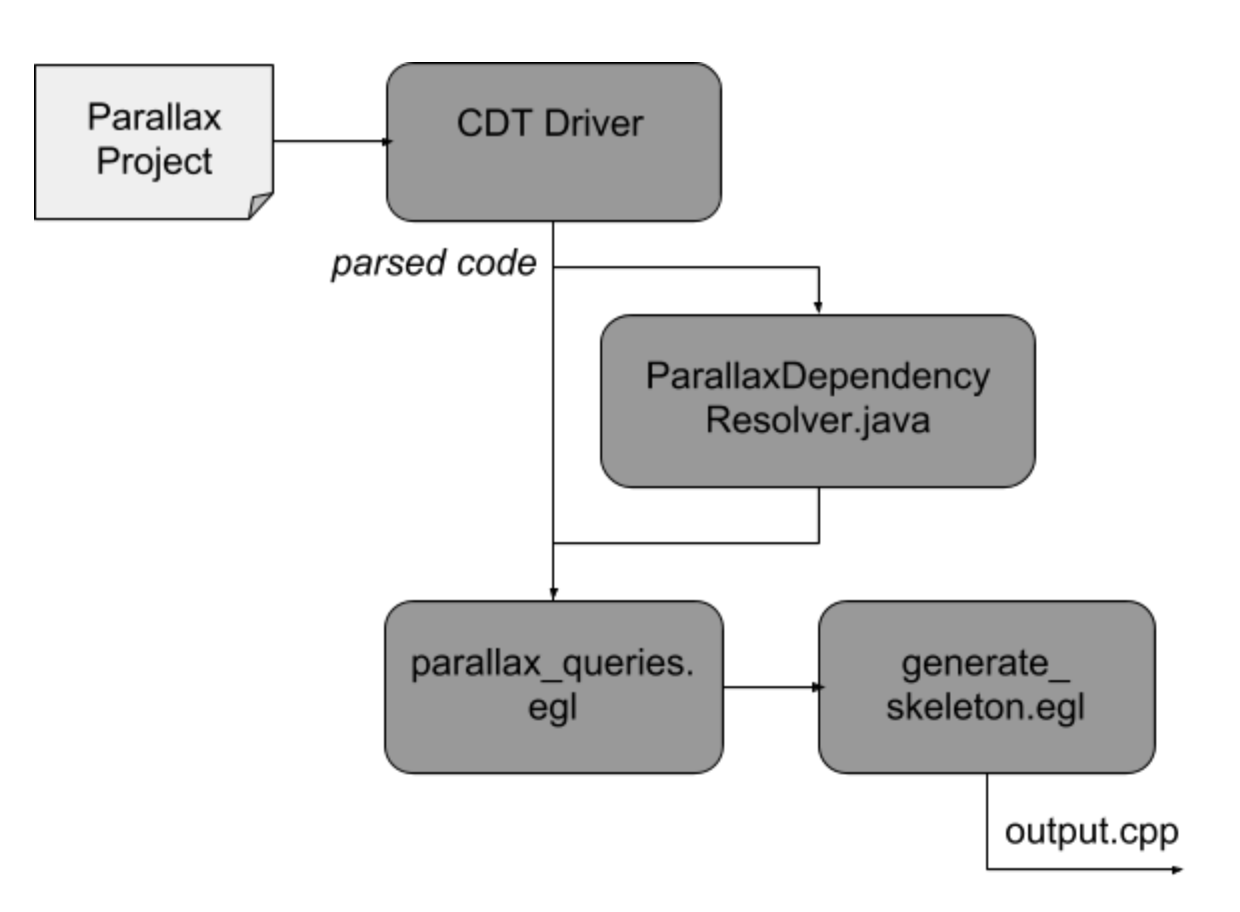
\includegraphics[width=0.8\linewidth]{graphics/parallax_project_analysis.png}
  \caption{A more detailed view of the Parallax project analysis component of the system.}
  \label{fig:parallax_analysis}
\end{figure}

\subsection{Design}
For a similar reason as in the Fritzing netlist analysis component, the information extracted in the Parallax project analysis stage is coordinated by an EOL file that is used by the Code Generation EGL transform. 

The logic contained in the Parallax Dependency Resolver Java code could have been implemented in the Parallax Queries EOL file. However, it would have been much more difficult to write. As such, a Java class encapsulating the required logic was created. This class is added to a plugin setup as in \parencite{eol_tool} so that it can be accessed from EOL as a Native type.

The Eclipse CDT Project provides a fully functional C and C++ Integrated Development Environment based on the Eclipse platform \parencite{eclipse_cdt}. The CDT Driver extends the Eclipse CDT Project, adding C/C++ support to the Epsilon framework (e.g. by providing support for C/C++ models) \parencite{cdt_driver}. These projects are used to support the analysis of the Parallax project.

\subsection{Implementation}
\begin{figure}[h!]
  \centering
  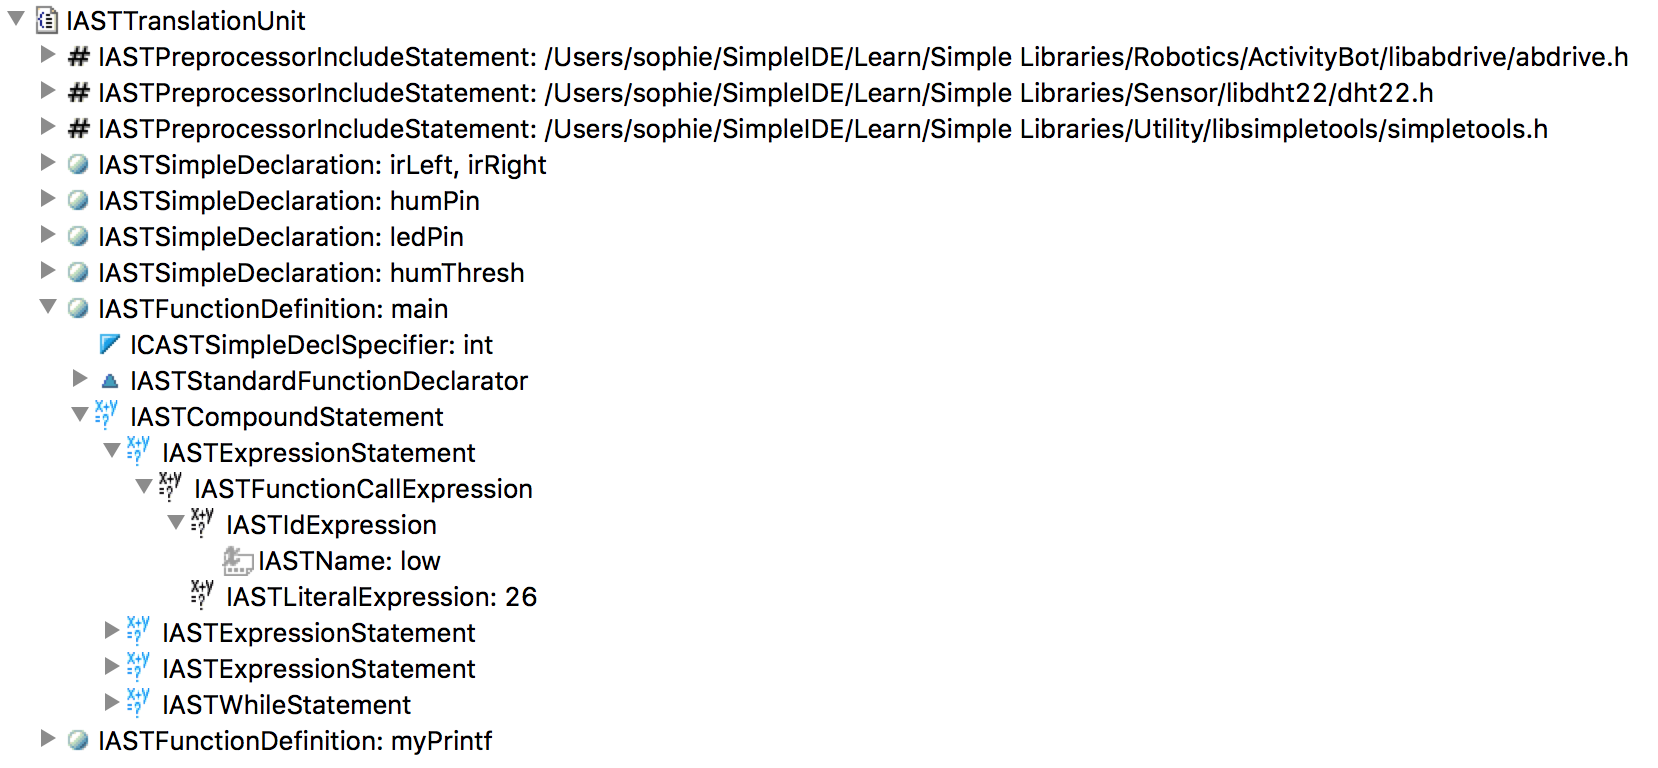
\includegraphics[width=0.8\linewidth]{graphics/ast_diagram.png}
  \caption{An example of a partially expanded AST for Parallax source code.}
  \label{fig:ast_diagram}
\end{figure}

CDT contains two parsers, for C and C++, which are able to generate an abstract syntax tree (AST) from source code \parencite{cdt_parsing}. Figure \ref{fig:ast_diagram} shows a partially expanded AST (more information on the structure of the AST can be found at \parencite{ast_structure}). The AST is generated for the input Parallax project and this is analysed to determine which constructs are part of Parallax libraries. These are then annotated in the generated code so that they can easily be replaced with equivalent functionality from the Arduino libraries. For example, functions from Parallax libraries are replaced with empty methods in the output file of the system. TODO directives within these empty methods make it clear they should be manually implemented. Figure \ref{fig:gen_stub} shows an example of a generated method.

\begin{figure}[h!]
  \centering
  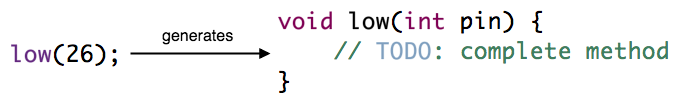
\includegraphics[width=0.8\linewidth]{graphics/generated_method_stub.png}
  \caption{An example of the empty method generated from a Parallax library function.}
  \label{fig:gen_stub}
\end{figure}

The constructs from Parallax libraries are identified as follows. The ParallaxDependencyResolver class extends the ASTVisitor class. This class implements the visitor design pattern and is the recommended method for traversing the AST based on \parencite{cdt_parsing}. This class is used to visit each $IASTNode$ in the AST (each construct in Figure \ref{fig:ast_diagram} is an $IASTNode$) and determine whether it belongs to a Parallax library. To determine whether a node  is declared/defined in within a Parallax library the following analysis is performed:
\begin{enumerate}
\item The index is created for the project. This contains all the binding information for the project. Since creating the index is a time-consuming process requiring parsing all the project code, resolving the bindings and writing them to the index, the index is only created once.
\item The $resolveBinding$ method is called on the $IASTName$ of the node. This returns an $IBinding$ instance.
\item The $IBinding$ is used to look up the $IIndexName$ for any declaration/definition of the node in the index.
\item The origin file can be found for this $IIndexName$. The file location is checked to see if it is contained within the directories containing the Parallax libraries. If so, it can be concluded that this node is part of a Parallax library and must be replaced in the output code.
\item If the node is determined to be part of the Parallax libraries, the declaration/definition of the node is collected.
\end{enumerate}

Once all the nodes have been processed, there will be a list of all the declarations/definitions that must be replaced in the output code. These are passed to the Code Generation EGL transform to create e.g. empty method stubs. Any other code is passed as is to the Code Generation EGL transform as is.

\section{Limitations}
This project is intended to be a proof-of-concept rather than a perfect implementation. As such, there are a few limitations in the approach which will be discussed below.

One of the main limitations of the system is the LibraryRanker for suggesting suitable Arduino libraries. Firstly, there's no guarantee that the Fritzing part names will actually be useful in searching for suitable libraries. For example, in Figure \ref{fig:lib_selection_ui} the name of the first part is shown as ``TSOP312.., 314..'' (this is actually an infrared receiver) - this doesn't give any indication of what the part is for and is unlikely to appear in any libraries as method names or in comments. Therefore, the suggestions for this part will be poor. However, it does provide a useful heuristic and creating a more accurate library suggestion system could easily be another project in itself and would therefore be infeasible in the time frame.

Another limitation is the assumption that the netlist input to the system is valid. For example, that the provided netlist is for a valid circuit and that it matches the configuration of the board that the generated code is intended to run on. As there is no easy way to check the correctness of this input, this is again outside the scope of the project.

A further limitation with the Fritzing netlist analysis component is that there is no mapping between pin variables declared in the source code and the variables generated for the target platform. For example, suppose the source code contains a variable \codeword{int humidityPin = 12} which is used in various method calls for accessing a humidity sensor. The Fritzing netlist analysis component generates a variable \codeword{int humidityPinGenerated = 6} which needs to replace \codeword{humidityPin}. There is currently no mechanism for automating this mapping and so pin variables will have to be replaced manually.

Additionally, due to time limitations the config file used for the Fritzing netlist analysis component does not contain information for all the components available in Fritzing. However, it would be fairly easy (albeit time-consuming) to update this with a more comprehensive file.

% TODO: assumption that there IS a mapping between libraries

%TODO: pin generation queries doesn't handle case where >1 sensor is connected to a board pin;
%TODO: would be easy to replace config w. hardcoded mapping between libs; no guarantee that previous library choices are reliable; no indication of how many times a library has previously been chosen;

% TODO: no backup for config file
%TODO: *** only migrates methods ->

\chapter{Evaluation}
This chapter aims to evaluate the software migration system against the requirements set out in Chapter \ref{req_gathering}. Section \ref{test_plan} outlines how this will be achieved followed by Sections \ref{test_cases}-\ref{eval_modifiability} describing the actual testing performed.

Tables \ref{table:case_study_sys_test_results} and \ref{table:case_study_func_test_results} summarise the results of the evaluation against the corresponding requirements. For each requirement from Chapter \ref{req_gathering} they indicate whether this requirement was met and include in the comments column which test case(s) or other analysis prove this is the case.

Finally, Sections \ref{test_summary} and \ref{eval_limits} summarise the testing and discuss the limitations of the project respectively.

\section{Test Plan} \label{test_plan}
The software migration system consists of three main components: Fritzing Netlist Analysis, Arduino Libraries Analysis and Parallax Source Analysis. Each of these components works independently of the others to generate outputs used by the Code Generation EGL transform. As such, each component can be tested separately to ensure the correct outputs are produced. Section \ref{test_cases} outlines the test cases used for this part of the evaluation.

The full system must then be evaluated against the requirements in Chapter \ref{req_gathering}. Case studies in Section \ref{eval_case_studies} are used to evaluate whether all requirements except S-2, NF-1 and NF-2 are met.

The requirements S-2, NF-1 and NF-2 concern the modifiability of the system. These requirements and whether they have been met are discussed in Section \ref{eval_modifiability}.
	
\section{Test Cases} \label{test_cases}
	
\subsection{Fritzing Netlist Analysis Test Cases}
The following test cases check that the Fritzing Netlist Analysis component generates pin variables as expected. Each test case contains a description of the goal of that particular test, the input netlist, expected variables and the actual output. Finally, Section \ref{fritzing_analysis_discussion} contains a discussion of the results of these tests.

\subsubsection{Test Case 1}
\begin{description}
\item[Description:] Check that a component with multiple pins is handled correctly.
\item[Input:] Netlist shown in Section \ref{lcd_netlist} for the diagram in Figure \ref{fig:lcd_test}.
\begin{figure}[h!]
  \centering
  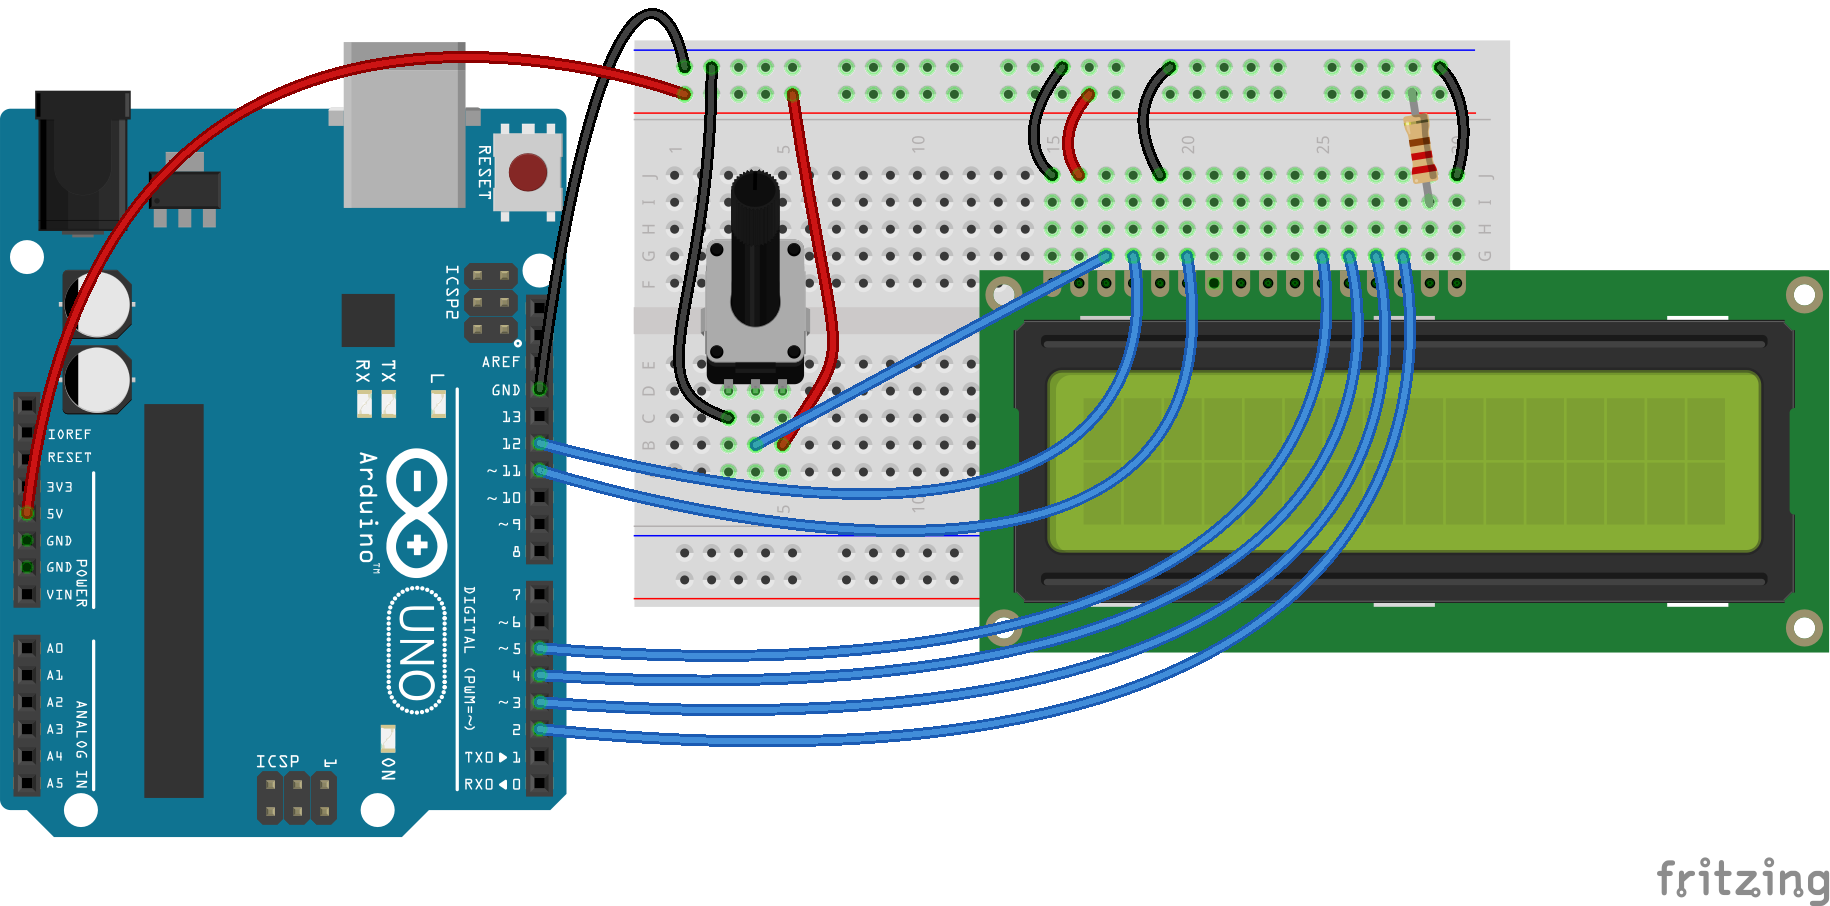
\includegraphics[width=0.5\linewidth]{graphics/LCD_test.png}
  \caption{Fritzing diagram for Fritzing netlist analysis test case 1.}
  \label{fig:lcd_test}
\end{figure}
\item[Expected Output:] lcd $\rightarrow$ 2, 3, 4, 5, 11, 12
\item[Actual Output:] See Figure \ref{fig:lcd_output}.
\begin{figure}[h!]
  \centering
  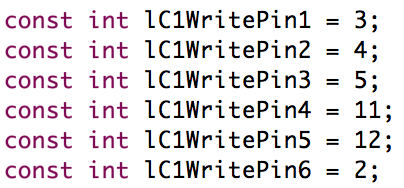
\includegraphics[width=0.4\linewidth]{graphics/lcd_test_output.png}
  \caption{Output of Fritzing netlist analysis test case 1.}
  \label{fig:lcd_output}
\end{figure}
\item[Result:] Test case passed
\end{description}

\subsubsection{Test Case 2}
\begin{description}
\item[Description:] Check that multiple components connected to one pin are handled correctly.
\item[Input:] Netlist shown in Section \ref{one_pin_netlist} for the diagram in Figure \ref{fig:one_pin_diagram}.
\begin{figure}[h!]
  \centering
  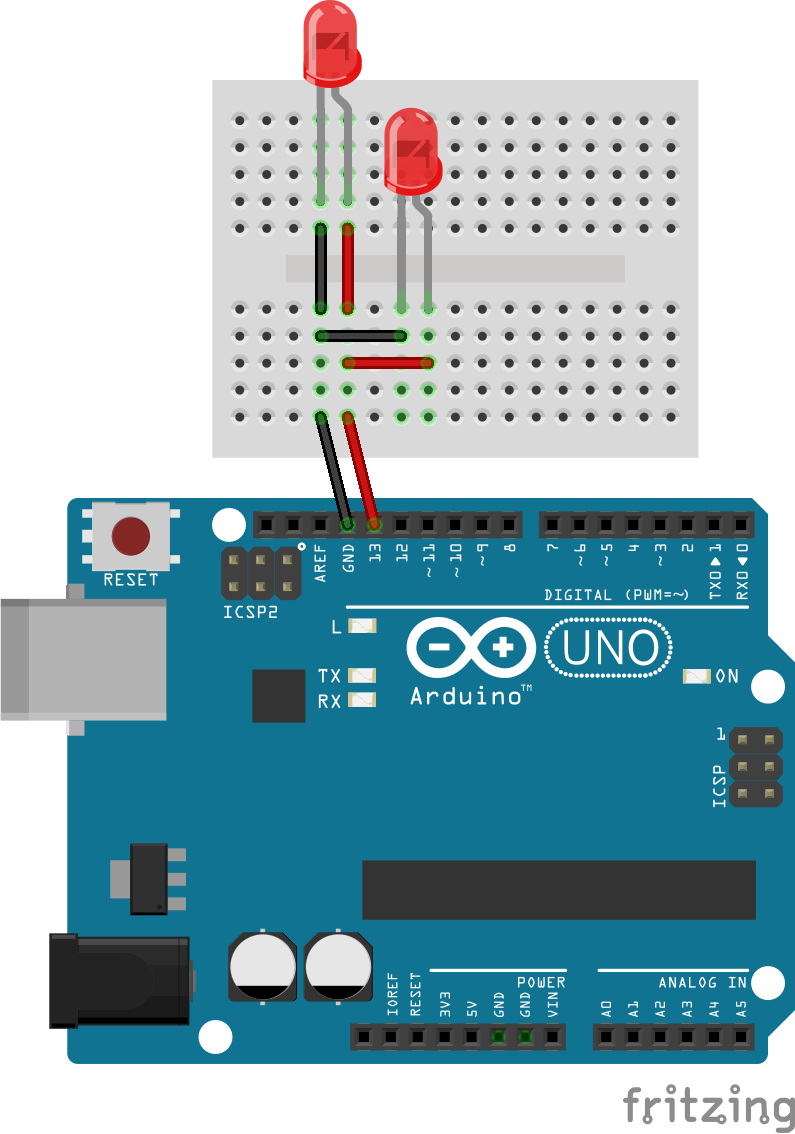
\includegraphics[width=0.3\linewidth]{graphics/One_Pin.png}
  \caption{Fritzing diagram for Fritzing netlist analysis test case 2.}
  \label{fig:one_pin_diagram}
\end{figure}
\item[Expected Output:] led1 $\rightarrow$ 13; led2 $\rightarrow$ 13
\item[Actual Output:] See Figure \ref{fig:one_pin_out}.
\begin{figure}[h!]
  \centering
  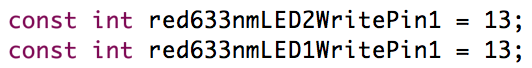
\includegraphics[width=0.5\linewidth]{graphics/one_pin_out.png}
  \caption{Output of Fritzing netlist analysis test case 2.}
  \label{fig:one_pin_out}
\end{figure}
\item[Result:] Test case passed
\end{description}

\subsubsection{Test Case 3} \label{fritz_tc3}
\begin{description}
\item[Description:] Check that a more complex netlist with many components is handled correctly. Additionally check that intermediate components between input/output parts (e.g. resistors) are ignored.

\item[Input:] Netlist shown in Section \ref{ir_hum_netlist} for the diagram in Figure \ref{fig:ir_hum_diagram}.
\begin{figure}[h!]
  \centering
  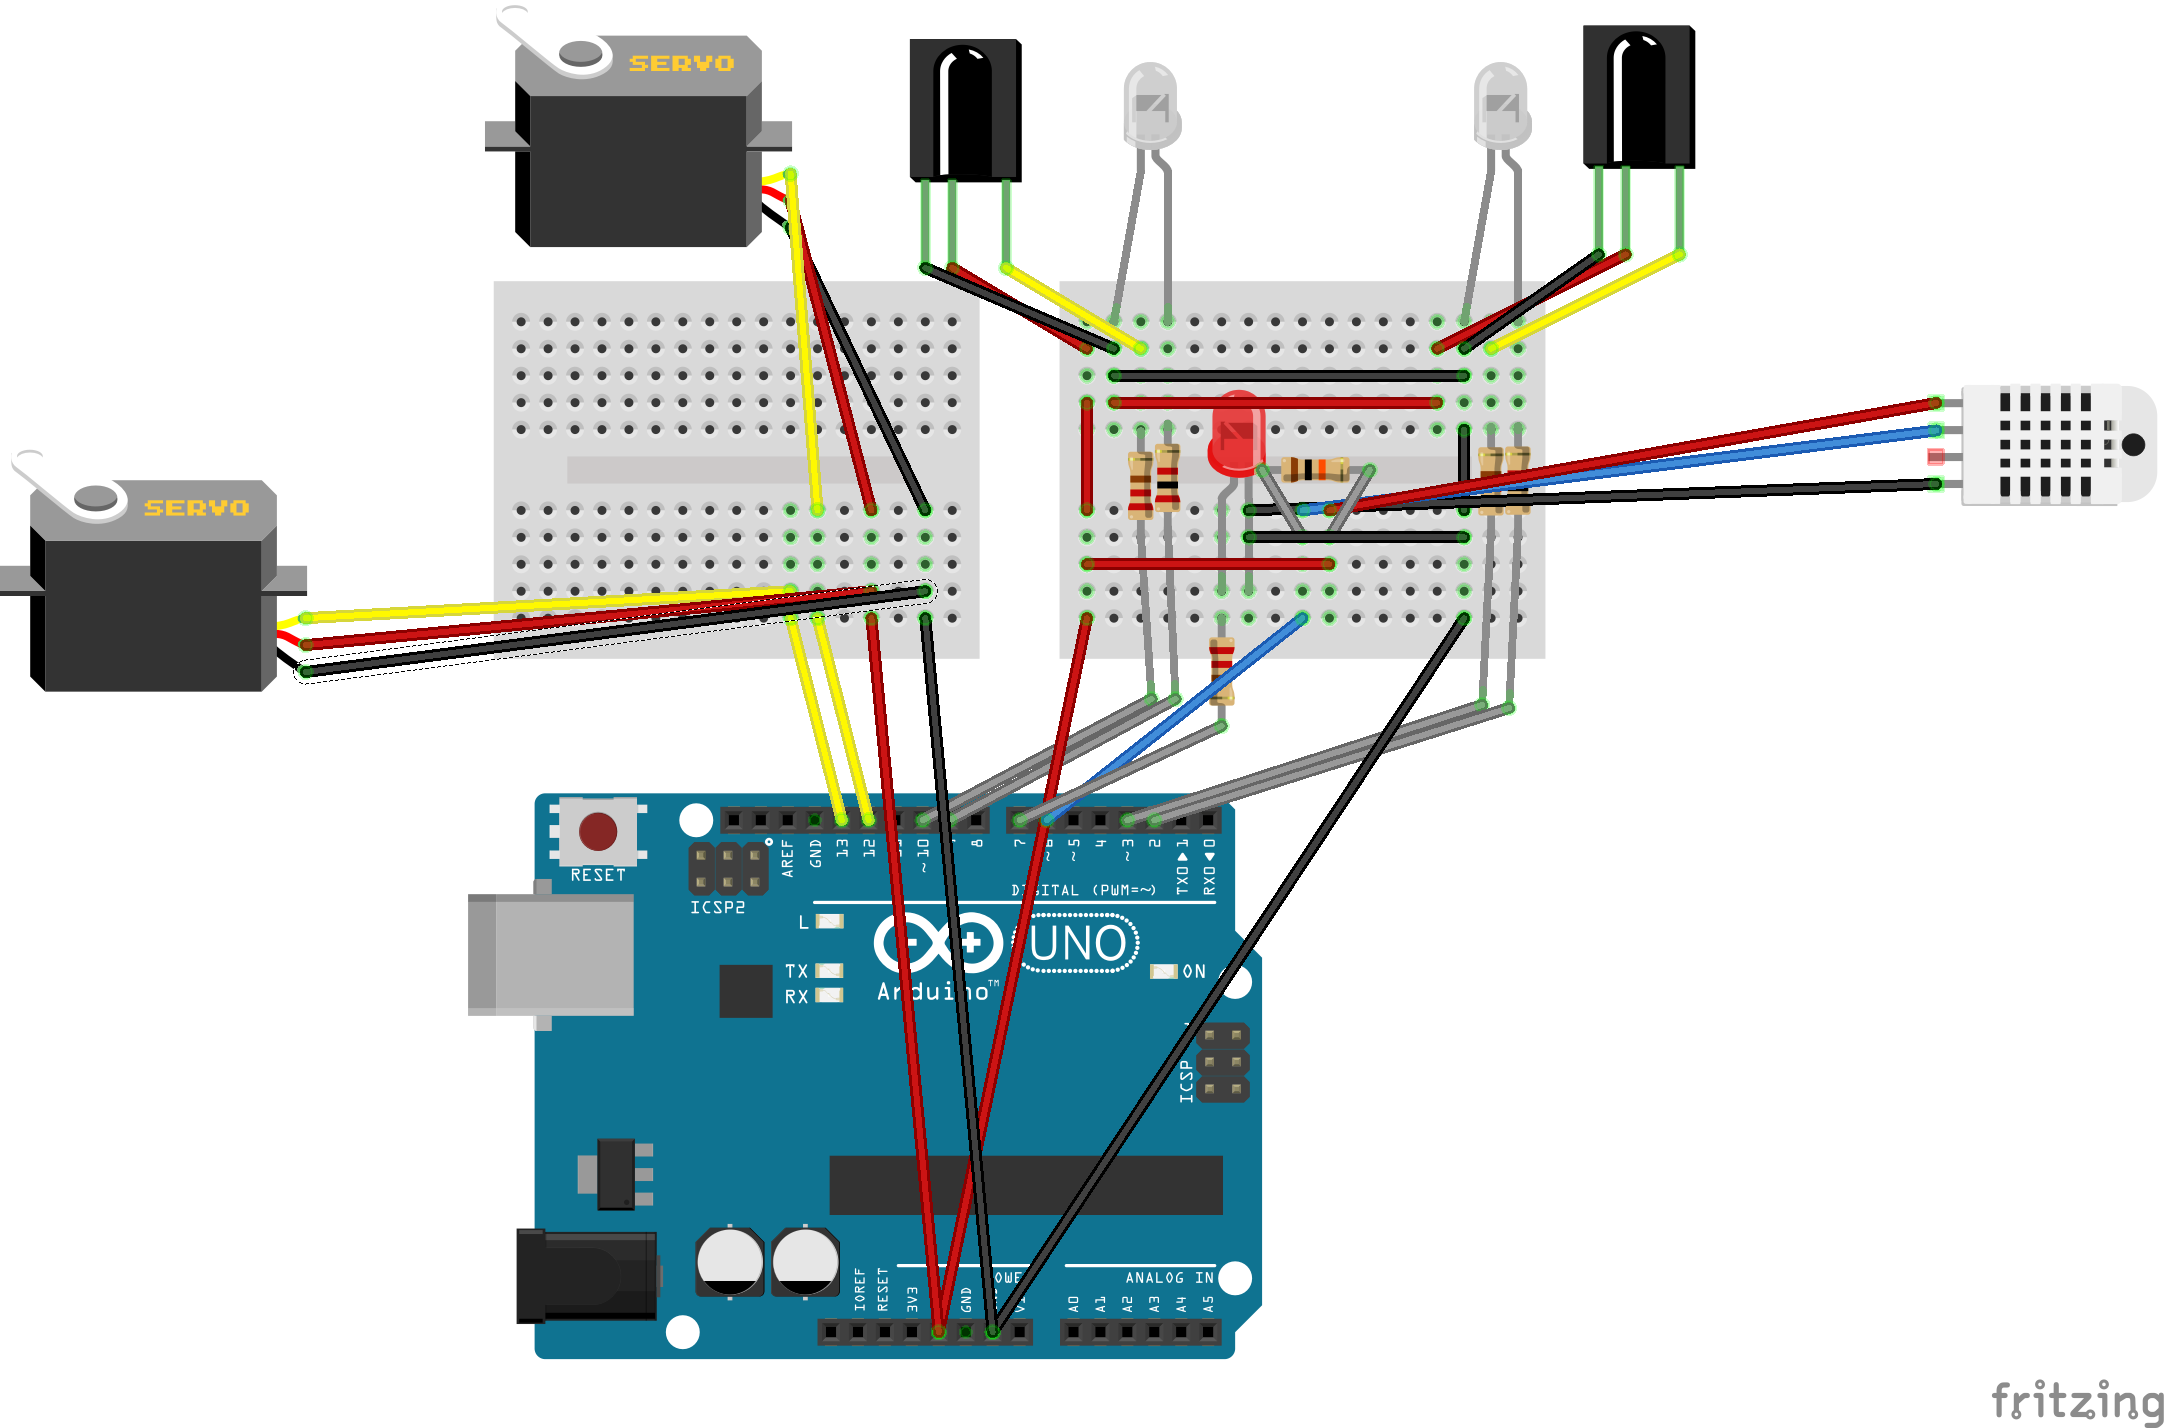
\includegraphics[width=0.7\linewidth]{graphics/ir_humidity_sensors.png}
  \caption{Fritzing diagram for Fritzing netlist analysis test case 3.}
  \label{fig:ir_hum_diagram}
\end{figure}
\item[Expected Output:] 
\begin{itemize}
\item IR receivers $\rightarrow$ 10, 3
\item IR LEDs $\rightarrow$ 9, 2
\item Servos $\rightarrow$ 13, 12
\item Red LED $\rightarrow$ 7
\item Humidity and temp. sensor $\rightarrow$ 6
\end{itemize}
\item[Actual Output:] See Figure \ref{fig:ir_hum_out}.
\begin{figure}[h!]
  \centering
  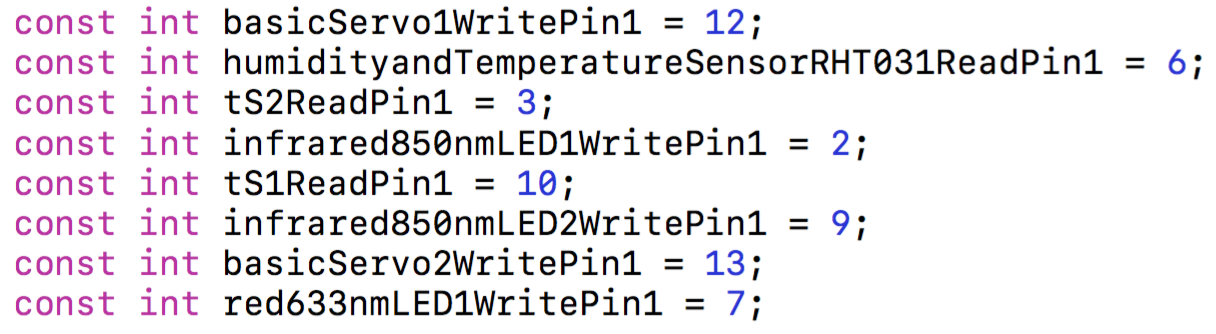
\includegraphics[width=0.7\linewidth]{graphics/cs1_gen_pins.png}
  \caption{Generated pin variables.}
  \label{fig:ir_hum_out}
\end{figure}
\item[Result:] Test case passed
\end{description}

\subsubsection{Discussion} \label{fritzing_analysis_discussion}
These test cases show the Fritzing netlist analysis component performs as expected. In addition, the generated variables have intelligible names for most cases. However, the variables \codeword{ts2ReadPin1/ts1ReadPin1} are not particularly useful. This is because the name of the IR receivers in Fritzing is ``TSOP312.., 314..'' and so this can't be used to generate a useful variable name. Additionally, the ``d'' has been cut off in the case of the LCD variables, for example, \codeword{lC1WritePin1}. This indicates more work needs to be done on the logic to generate the variable names. 

\subsection{Arduino Library Suggestion Test Cases}
The following test cases evaluate the quality of the output from the Arduino libraries suggestion component. Three circuit parts that require the use of Arduino libraries have been chosen and this component has been used to generate a list of candidate libraries. For each component, the suggestions are inspected to determine the rank of the expected library. Section \ref{arduino_lib_discussion} discusses the results of these test cases.

\subsubsection{Test Case 1}
\begin{description}
\item[Input:] LCD Screen
\item[Expected Library:] \codeword{LiquidCrystal.h}
\item[Actual Output:] See Figure \ref{fig:lib_suggest_lcd}.
\begin{figure}[h!]
  \centering
  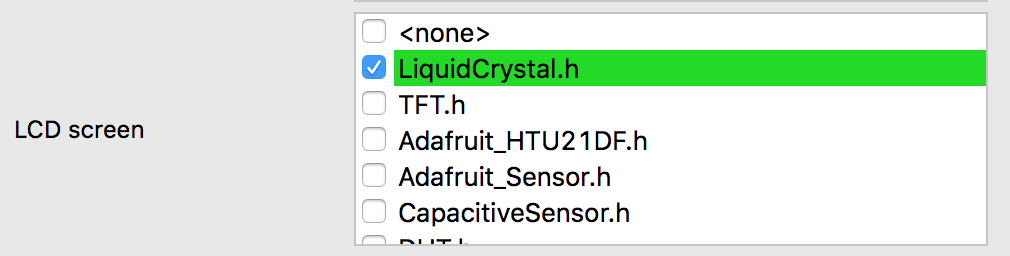
\includegraphics[width=0.5\linewidth]{graphics/lib_suggest_lcd.png}
  \caption{Output of Arduino library suggestion test case 1.}
  \label{fig:lib_suggest_lcd}
\end{figure}
\end{description}

\subsubsection{Test Case 2} \label{arduino_tc2}
\begin{description}
\item[Input:] Humidity and temperature sensor (DHT22)
\item[Expected Library:] \codeword{DHT.h}
\item[Actual Output:] See Figure \ref{fig:lib_suggest_humidity}.
\begin{figure}[h!]
  \centering
  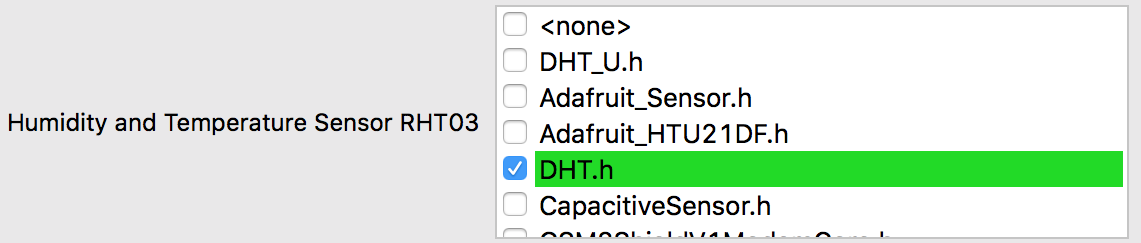
\includegraphics[width=0.5\linewidth]{graphics/lib_suggest_humidity.png}
  \caption{Output of Arduino library suggestion test case 2.}
  \label{fig:lib_suggest_humidity}
\end{figure}
\end{description}

\subsubsection{Test Case 3} \label{arduino_tc3}
\begin{description}
\item[Input:] Servo
\item[Expected Library:] \codeword{Servo.h}
\item[Actual Output:] See Figure \ref{fig:lib_suggest_servo}.
\begin{figure}[h!]
  \centering
  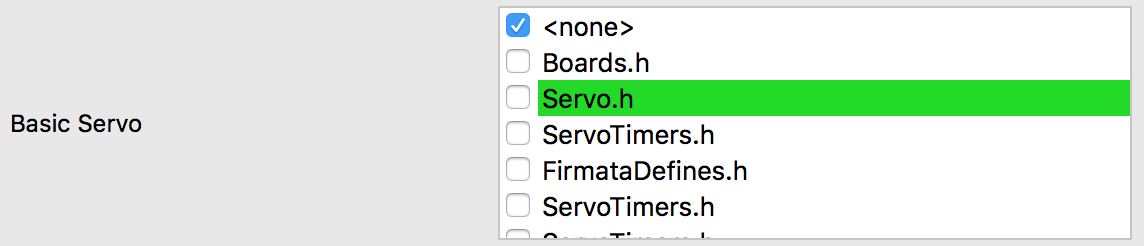
\includegraphics[width=0.5\linewidth]{graphics/lib_suggest_servo.png}
  \caption{Output of Arduino library suggestion test case 3.}
  \label{fig:lib_suggest_servo}
\end{figure}
\end{description}

\subsubsection{Discussion} \label{arduino_lib_discussion}
For all three test cases the correct libraries were shown in the top 5 suggestions showing that, in this case, LibraryRanker provides a useful heuristic for narrowing down the libraries for the target platform code. The ranking algorithm proved particularly effective for the LCD display component with the appropriate \codeword{LiquidCrystal.h} library being ranked top. Although the correct library was only ranked fourth in the case of the humidity and temperature sensor, the more highly suggested libraries are all for humidity/temp. sensors just not the specific \codeword{DHT22} sensor used in this circuit.

A potential issue with the ranking algorithm is highlighted by the servo test case. The \codeword{Boards.h} library is ranked higher than \codeword{Servo.h} as it contains macro definitions for variables such as \codeword{MAX_SERVOS} for many different types of board (e.g. Arduino Mega, Primo etc.) and therefore the term ``servo'' appears many times, contributing to a higher \textbf{TF-IDF} rank. A potential improvement to the ranking heuristic would also take file size into account e.g. consider the proportion of the file containing the term ``servo'' as opposed to the raw count.

\subsection{Parallax Source Code Analysis Test Cases} \label{pscatc}
The expected behaviour for code generation is:
\begin{itemize}
\item Parallax library include statements \textit{are not} present in the output
\item Any other library include statements \textit{are} present in the generated code
\item Empty methods with TODO directives are generated for any Parallax library methods used in the input code
\item Code from the main method outside of the \codeword{while(1)} loop in the input is copied to a \codeword{setup()} method in the output
\item Code from the \codeword{while(1)} loop in the input is copied to the \codeword{loop()} method of the output
\item Any other methods defined in the input are copied to the output
\item Global variables in the input are copied to the output
\end{itemize}
The test case in Section \ref{parallax_tc1} checks that the Parallax source code analysis component generates code as expected.

\subsubsection{Test Case 1} \label{parallax_tc1}
\begin{description}
\item[Description:] The input source code contains a mixture of Parallax library methods and other functions as well as global variables, user-defined methods and include statements for non-Parallax libraries. This test case checks all the criteria for a successful migration (as discussed in Section \ref{pscatc}) are met.
\item[Input:] The source code in Appendix \ref{ir_hum_parallax_in}.
\item[Expected Output:] 
\begin{enumerate}
\item Methods generated with the following signatures:
\begin{itemize}
\item \codeword{void drive_setRampStep(int stepsize)}
\item \codeword{void drive_rampStep(int left, int right)}
\item \codeword{int input(int pin)}
\item \codeword{void high(int pin)}
\item \codeword{void low(int pin)}
\item \codeword{void freqout(int pin, int msTime, int frequency)}
\item \codeword{char dht22_read(int dht_pin)}
\item \codeword{int dht22_getTemp(char temp_units)}
\item \codeword{int dht22_getHumidity()}
\end{itemize}
\item Only \codeword{stdio.h} include in output.
\item The global variables \codeword{int irLeft, irRight;}; \codeword{int humPin = 6;}; \codeword{int ledPin = 8;} and \codeword{float humThresh = 25.0;} are present in the output.
\item The statements \codeword{low(26);}; \codeword{low(27);} and \codeword{drive_setRampStep(12);} are included in the \codeword{setup()} method of the output. 
\item All other statements in the main method of the input are in the \codeword{loop()} method of the output. 
\item The \codeword{myPrintf} method from the input is copied to the output.
\end{enumerate}
\item[Actual Output:] See Appendix \ref{parallax_tc1_out}.
\item[Result:] Test case passed.
\end{description}

\section{Case Studies} \label{eval_case_studies}
The following case studies are used to evaluate whether the requirements set out in Chapter \ref{req_gathering} have been met. The first case study in Section \ref{cs1} demonstrates the operation of the system when provided with correct inputs and is used to evaluate requirements S-1, S-4, S-5, F-1, F-2, F-5, NF-3 and NF-4. The second and third case studies (in sections \ref{cs2} and \ref{cs3}) are used to evaluate the system when there are errors in the migration process. These case studies are used to evaluate requirements F-3 and F-4 respectively. A summary of the results of these case studies along with the corresponding requirements are contained in tables \ref{table:case_study_sys_test_results} and \ref{table:case_study_func_test_results}.

\subsection{Case Study 1 (CS-1)} \label{cs1}
Figure \ref{fig:ir_hum_diagram} shows the Fritzing diagram for the target platform in CS-1. The source code, Fritzing netlist and generated code for this case study can be viewed in Appendices \ref{ir_hum_parallax_in}, \ref{ir_hum_netlist} and \ref{cs1_out} respectively. For this case study, the correct functioning of the Fritzing netlist analysis, Arduino libraries suggestion and Parallax source code analysis components have been evaluated in the earlier sections \ref{fritz_tc3}, \ref{arduino_tc2}/\ref{arduino_tc3} and \ref{parallax_tc1} respectively. The migrated code (i.e. the output code from the system with manual additions) is shown in Appendix \ref{cs1_migrated}.

\subsubsection{Description} \label{cs1_description}
The source code and circuit uses infrared receivers/LEDs to detect and move around its surroundings using servo motors. Periodically, a humidity reading is taken from the humidity/temperature sensor. If this is above some threshold, an LED lights up. When connected to a computer, the humidity and temperature readings can be displayed to the console. Since Parallax only supports a subset of C, in order to write to the console a function myPrintf is defined in the source code. This performs the same function as the standard libraries' printf.

This case study is used to demonstrate the migration of code for components that require different complexities of mapping between the source and target platforms. Firstly, it is fairly simple to map between the libraries for the humidity and temperature sensor. 

In the Parallax source, this sensor can be used as:
\begin{verbatim}
#include "dht22.h"

dht22_read(sensorPin);        // Get most recent readings
dht22_getHumidity();          // Get humidity reading
dht22_getTemp(CELSIUS);       // Get temperature reading
\end{verbatim}

To use the same functionality in the Arduino code requires the following:
\begin{verbatim}
#include "DHT.h"

DHT humiditySensor(DHTPIN, DHTTYPE); // Setup
humiditySensor.readHumidity();       // Get humidity reading
humiditySensor.readTemperature();    // Get temperature reading
\end{verbatim}

Aside from some small differences in how the sensors are initialised, there is an almost exact mapping between the methods for reading humidity/temperature values. 

Mapping between methods to use the servos is more difficult. For example, to control the servos in Parallax, you can provide the speed to each servo in ticks per second (where a tick is $\frac{1}{64}$ of a wheel rotation). The Parallax libraries also include methods to gradually accelerate to a specified speed (e.g. \codeword{drive_RampStep}. On the other hand, the Arduino libraries control the servos using pulse width (see \parencite{pulse_width} for more information on how this is used to control servos). See below for an example of how servos are controlled in Parallax compared to Arduino.
\begin{verbatim}
/* Parallax */
#include "abdrive.h"

// Perform two servo rotations per second
// Note we do not need to set up pins for the servos in Parallax
drive_rampStep(128 /*left*/, 128 /*right*/); 

/* Arduino */

Servo servoLeft, servoRight;

// Setup servo pins
servoLeft.attach(13);
servoRight.attach(12);

servoLeft.writeMicroseconds(1600);
servoRight.writeMicroseconds(1600);
delay(20); 
\end{verbatim}

\subsubsection{Analysis}
Firstly, the system was successful in demonstrating that, provided with correct inputs, it is able to generate code (i.e. Appendix \ref{cs1_out}) that with manual additions (i.e. Appendix \ref{cs1_migrated}) can be run on the target platform, consequently satisfying requirement S-1.
 
Two types of compile-time errors were present in the generated output (see Appendix \ref{cs1_out}) from the migration system. Firstly, a macro definition from the Parallax \codeword{dht22} library (\codeword{CELSIUS}) caused an error as it was not defined in the generated output (see Figure \ref{fig:celsius_error}). Other than this compile time error, there was no indication that this variable needed to be replaced in the generated code which is in conflict with requirements S-4/F-5. However, other than this small issue, the methods that needed to be completed were clearly marked.
\begin{figure}[h!]
  \centering
  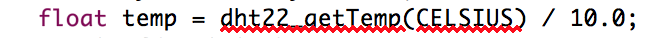
\includegraphics[width=0.7\linewidth]{graphics/celsius_error.png}
  \caption{Compile error due to header macro definition.}
  \label{fig:celsius_error}
\end{figure}

Figure \ref{fig:celsius_ast} shows the AST of the source code for this declaration. Although \codeword{CELSIUS} is used in the code, this is resolved to the literal expression having a value of 0 in the AST. As such, there is no way to tell from the AST that this value comes from a definition in a library file. One solution would be to copy all the macro definitions from the includes in the Parallax code. However, this could become very messy and increase the file size a lot particularly when there are many included files. A better solution would require creating a parser that would indicate these macros within the AST but this is outside the scope of this project.

\begin{figure}[h!]
  \centering
  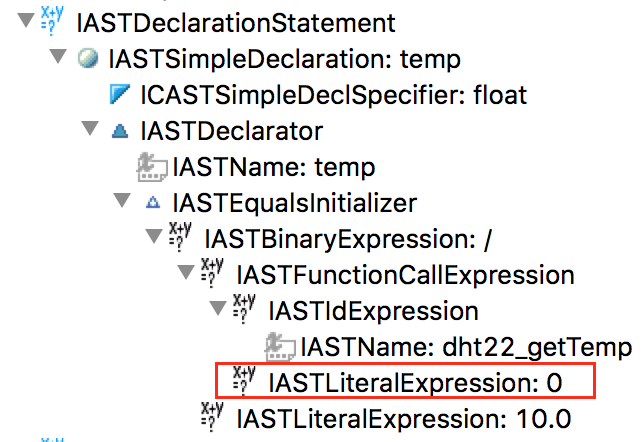
\includegraphics[width=0.5\linewidth]{graphics/celsius_ast.png}
  \caption{AST for the declaration using a macro definition. The value is resolved to a literal expression (highlighted in red).}
  \label{fig:celsius_ast}
\end{figure}

The second type of compile-time error is due to no return types as can be seen in Figure \ref{fig:return_type_error}. It would be fairly easy to add default return values. However, this compile-time error can work as an extra indication that this method needs completing manually and so it is useful to leave this procedure as it is.

\begin{figure}[h!]
  \centering
  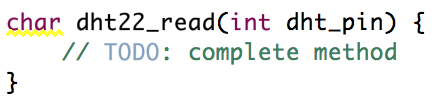
\includegraphics[width=0.5\linewidth]{graphics/return_type_error.png}
  \caption{Compile error due to no return.}
  \label{fig:return_type_error}
\end{figure}

As these errors were resolved with the manual additions required for migration, it was demonstrated that requirement F-2 was satisfied and the code in Appendix \ref{cs1_migrated} was able to be deployed on the Arduino without errors.

The size of the Parallax source code was 1,506 bytes compared to 2,156 bytes for the generated code and 2,922 bytes for the manually completed code. As such, the migrated code is roughly twice the size of the input. However, some unused functions have been left in the migrated code for demonstration purposes so the migrated code could be made smaller. It should be expected that there will be a constant factor increase in the size of the migrated code since empty methods are generated for each of the Parallax library functions in the source code. In the worst case, each line of the input will make use of a Parallax library function, requiring three generated lines of code in the output (method declaration; TODO statement; closing bracket). There may also be additional lines added for generated pin variables and target platform include statements. However, the size of these additions is likely to be small compared to the size of generated methods. Therefore, an upper bound on the generated code (without manual additions) is 3L where L is the number of lines in the input. For most cases this would be an acceptable increase in size and so NF-3 is satisfied. However, of course this depends on the requirements for the particular application. Furthermore, the size of the output depends on the mappings between library functions for the source and target platforms. For example, I found that to perform the same functionality using Arduino libraries tends to require more lines of code since setup is generally made more explicit than when using Parallax libraries (e.g. consider the servo code in Section \ref{cs1_description}). As such, it may be expected that programs rewritten directly for the target platform may be larger anyway without the use of this migration system.

Based on an inspection of the application run on both the source and target platforms, there was no perceptible difference in performance and so requirements S-5/NF-4 are satisfied. The only potential reduction in performance (other than platform differences) could come from the use of additional method calls from the generated methods. However, compilers optimized for speed can inline functions in this case so that this does not occur. Otherwise, the difference is likely to be negligible unless there is a cache miss \parencite{function_call_performance}. Other than this, differences in performance are likely to be much more dependent on the efficiency of the corresponding platform libraries and the hardware specifications for the microcontrollers themselves.

Between the source and target applications there are some minor differences in behaviour because of the differences in libraries. For example, the servos do not accelerate when running the code on the Arduino as they do on the Parallax board since there is no equivalent function in the Arduino libraries (see Section \ref{cs1_description}). Other than this, from manual inspection, the migrated code performs the same functionality as the source code (i.e. using infrared LEDs/receivers to maneuver and periodically take humidity/temp. readings etc.) and so requirement F-1 is met.

Overall, with some minor exceptions, this case study has demonstrated that requirements S-1, S-4, S-5, F-1, F-2, F-5, NF-3 and NF-4 have been met.

\subsection{Case Study 2 (CS-2)} \label{cs2}
%TODO: case study to eval F-3 (display errors when source code can't be migrated)

\subsection{Case Study 3 (CS-3)} \label{cs3}
%TODO: case study to eval F-4 (indicate errors during migration process)

\section{Evaluation of Modifiability} \label{eval_modifiability}
%TODO: discuss how design of system supports modification

%TODO: add results in table (e.g. tick and state satisfied because of CS-1)
\newgeometry{left=3cm,bottom=2cm, top=3cm, right=2.5cm, footskip=0.2cm}
\begin{landscape}
\begin{table*}[h!]\centering
\ra{1.3}
  \begin{tabular}{@{}p{0.1\textwidth}p{0.15\textwidth}p{0.3\textwidth}p{0.15\textwidth}p{0.3\textwidth}@{}} \toprule 
  \textbf{ID} & \textbf{Priority} & \textbf{Description} & \textbf{Satisfied} & \textbf{Comments} \\
  \midrule
  S-1 & M & Users can provide the system with the source code for a Parallax Propeller Activity Board and target code for the Arduino Uno will be generated. & \checkmark & - \\ 
  S-2 & M & Users can easily adapt the system to support migration of software between different microprocessors. & - & - \\
  S-3 & S & Users can easily determine sources of errors when using the system. & - & - \\
  S-4 & S & Users can easily identify areas of the target code that cannot automatically be migrated and must be manually completed. & - & - \\
  S-5 & S & The performance of the migrated code is not significantly worse than the source application. & - & - \\
  \bottomrule
  \end{tabular}
\caption{Case Study System Test Results}
\label{table:case_study_sys_test_results}
\end{table*}

\clearpage

\ra{1.3}
  \begin{longtable}{@{}p{0.06\textwidth}p{0.05\textwidth}p{0.3\textwidth}p{0.3\textwidth}p{0.05\textwidth}p{0.24\textwidth}@{}} \toprule 
  \textbf{ID} & \textbf{P} & \textbf{Description} & \textbf{Acceptance Criteria} &\textbf{S} & \textbf{Comments} \\
  \midrule
      F-1 & M & The target microcontoller running the migrated code (potentially with manual additions) displays the same behaviour as the source microcontroller, provided the source code is valid. & Manual inspection of the migrated application confirms the behaviour is the same as the source application. & - & - \\
  F-2 & M & The migrated code deploys without errors on the target microcontroller if the provided source code is valid. & Manual inspection of the migration process confirms a valid source application can be migrated without errors. & - & - \\
  F-3 & S & The system displays appropriate errors when the source code cannot be migrated (e.g. there are errors in the source code or hardware incompatibilities). & Errors are thrown when invalid source code is provided to the migration process. & - & - \\  
  F-4 & S & The system clearly indicates any errors that have occurred during its use (e.g. the migration process fails). & Errors are thrown if the migration process fails. The errors clearly indicate the source of the problem. & - & - \\
  F-5 & S & The system should indicate any parts of the code that must be manually completed. & Manual inspection of the migrated code confirms that all parts of the code that must be manually completed are clearly indicated (e.g. by TODO directives). & - & - \\
    NF-1 & M & The system should be easy to adapt to support migration between different microcontrollers. & Manual inspection of the system should indicate that it is easy to adapt. For example, if the system is based on an established MDE framework it will be easier to adapt as there will be more documentation available. & - & - \\
  NF-2 & S & The system should display a high-level of encapsulation. & Manual inspection of the system should indicate measures have been taken to facilitate encapsulation. For example, separation of hardware-dependent parts of the code. & - & - \\
  NF-3 & S & The migrated code should not be significantly larger than the source code. & Migrated code is of a size acceptable to the stakeholder. & - & - \\
  NF-4 & S & The migrated code should exhibit similar performance to the source code. & Migrated code runs in a duration acceptable for the stakeholder. & - & - \\
    \bottomrule
\caption{Case Study Functionl/Non-Functional Test Results}
\label{table:case_study_func_test_results}
  \end{longtable}
\end{landscape}

\restoregeometry

\section{Test Summary} \label{test_summary}
%TODO: complete test summary incl. summary of current issues
\subsection{Current Issues}
\section{Limitations} \label{eval_limits}
%TODO: complete limitations - internal, external, construct, conclusion validity


\chapter{Conclusion}
%TODO
%TODO discuss effort of testing
%TODO: further work - analyze includes to map between libraries e.g. "abdrive.h" -> "Servo.h"
%TODO: ranking libs -> larger libraries more likely to be ranked higher e.g. boards.h has many references to servos because it contains defs for each board
%TODO: copy across comments for methods stubs -> otherwise have to lookup what function does
%TODO: migrate between classes and typedefs

\printbibliography

\begin{appendices}
\chapter{Fritzing Netlist Analysis Test Inputs}
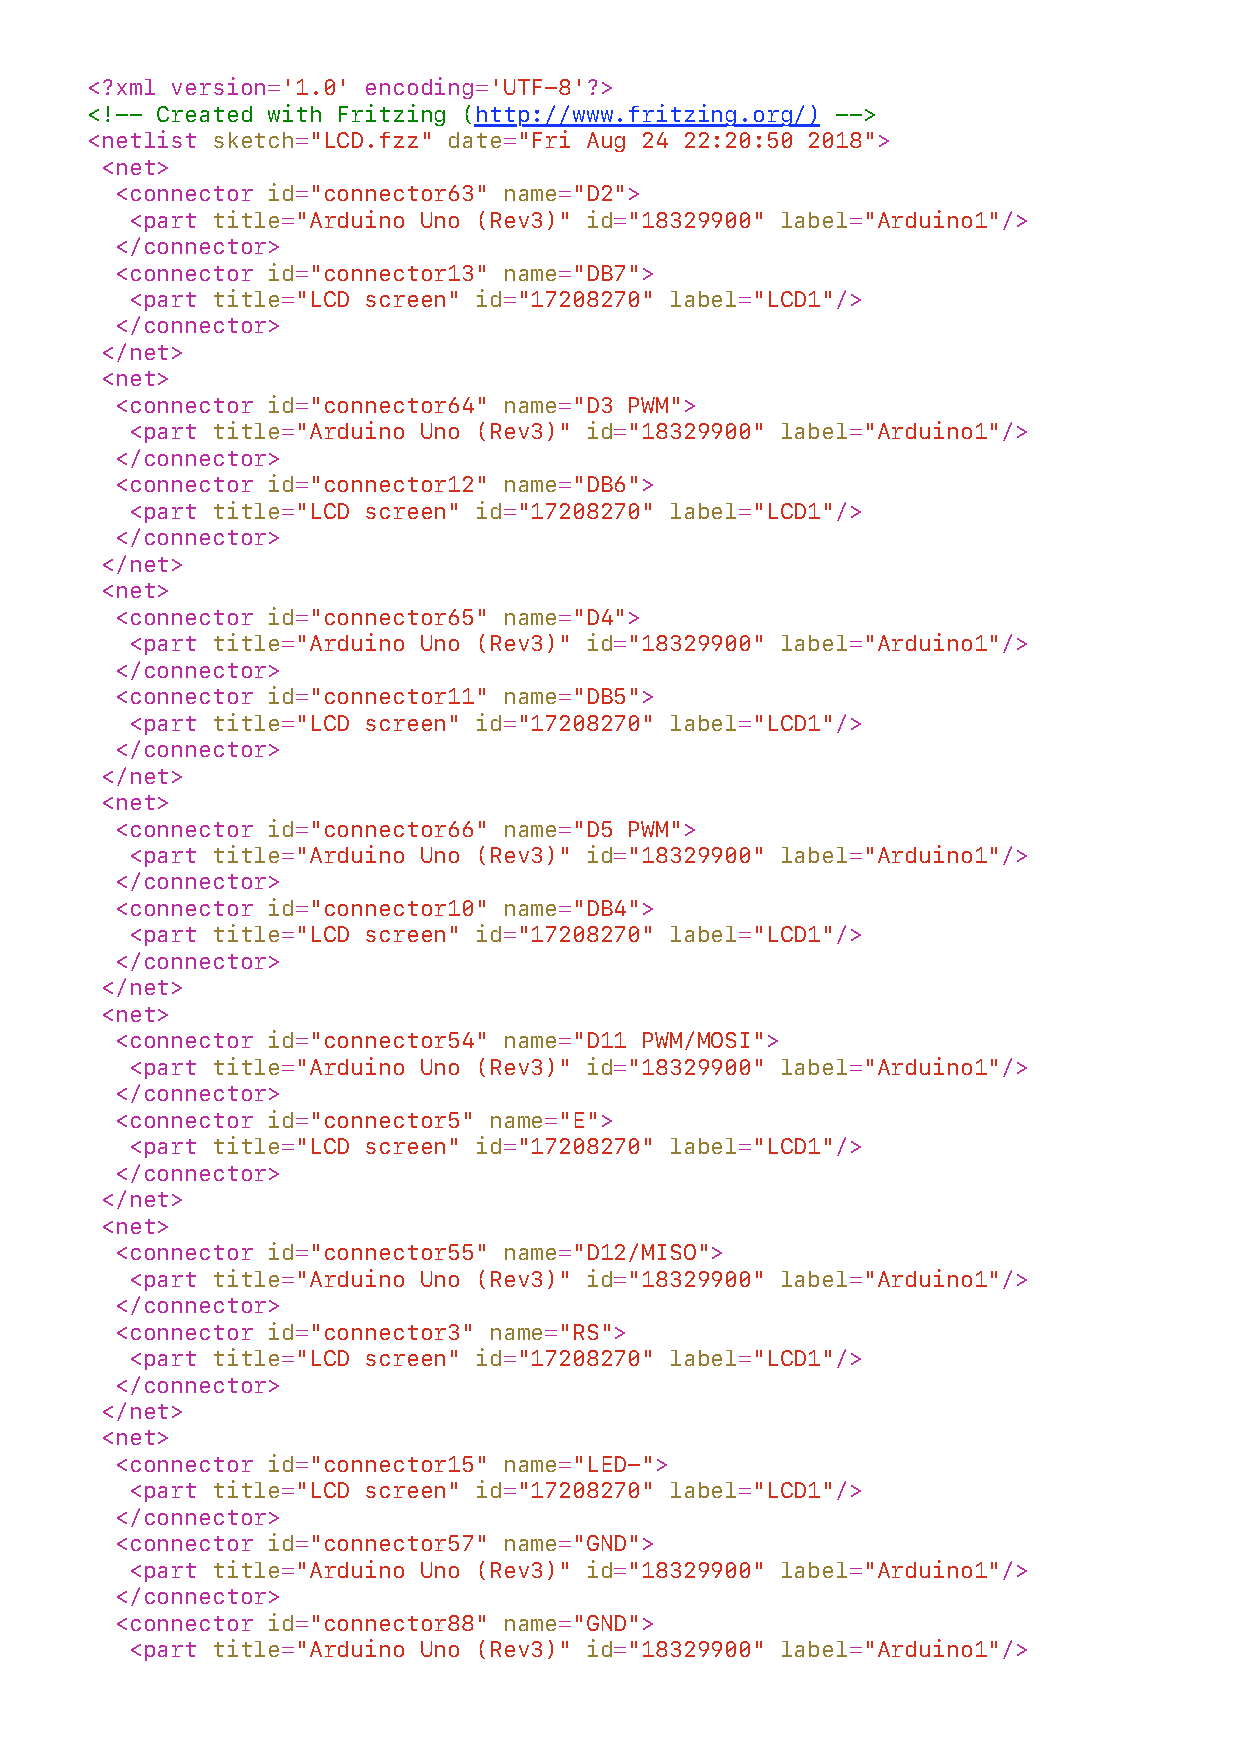
\includepdf[pages=1,scale=0.75, pagecommand=\section{Test Case 1 Netlist}\label{lcd_netlist}]{graphics/LCD_netlist.pdf}
\includepdf[pages=2-,scale=0.75, pagecommand={}]{graphics/One_Pin.pdf}
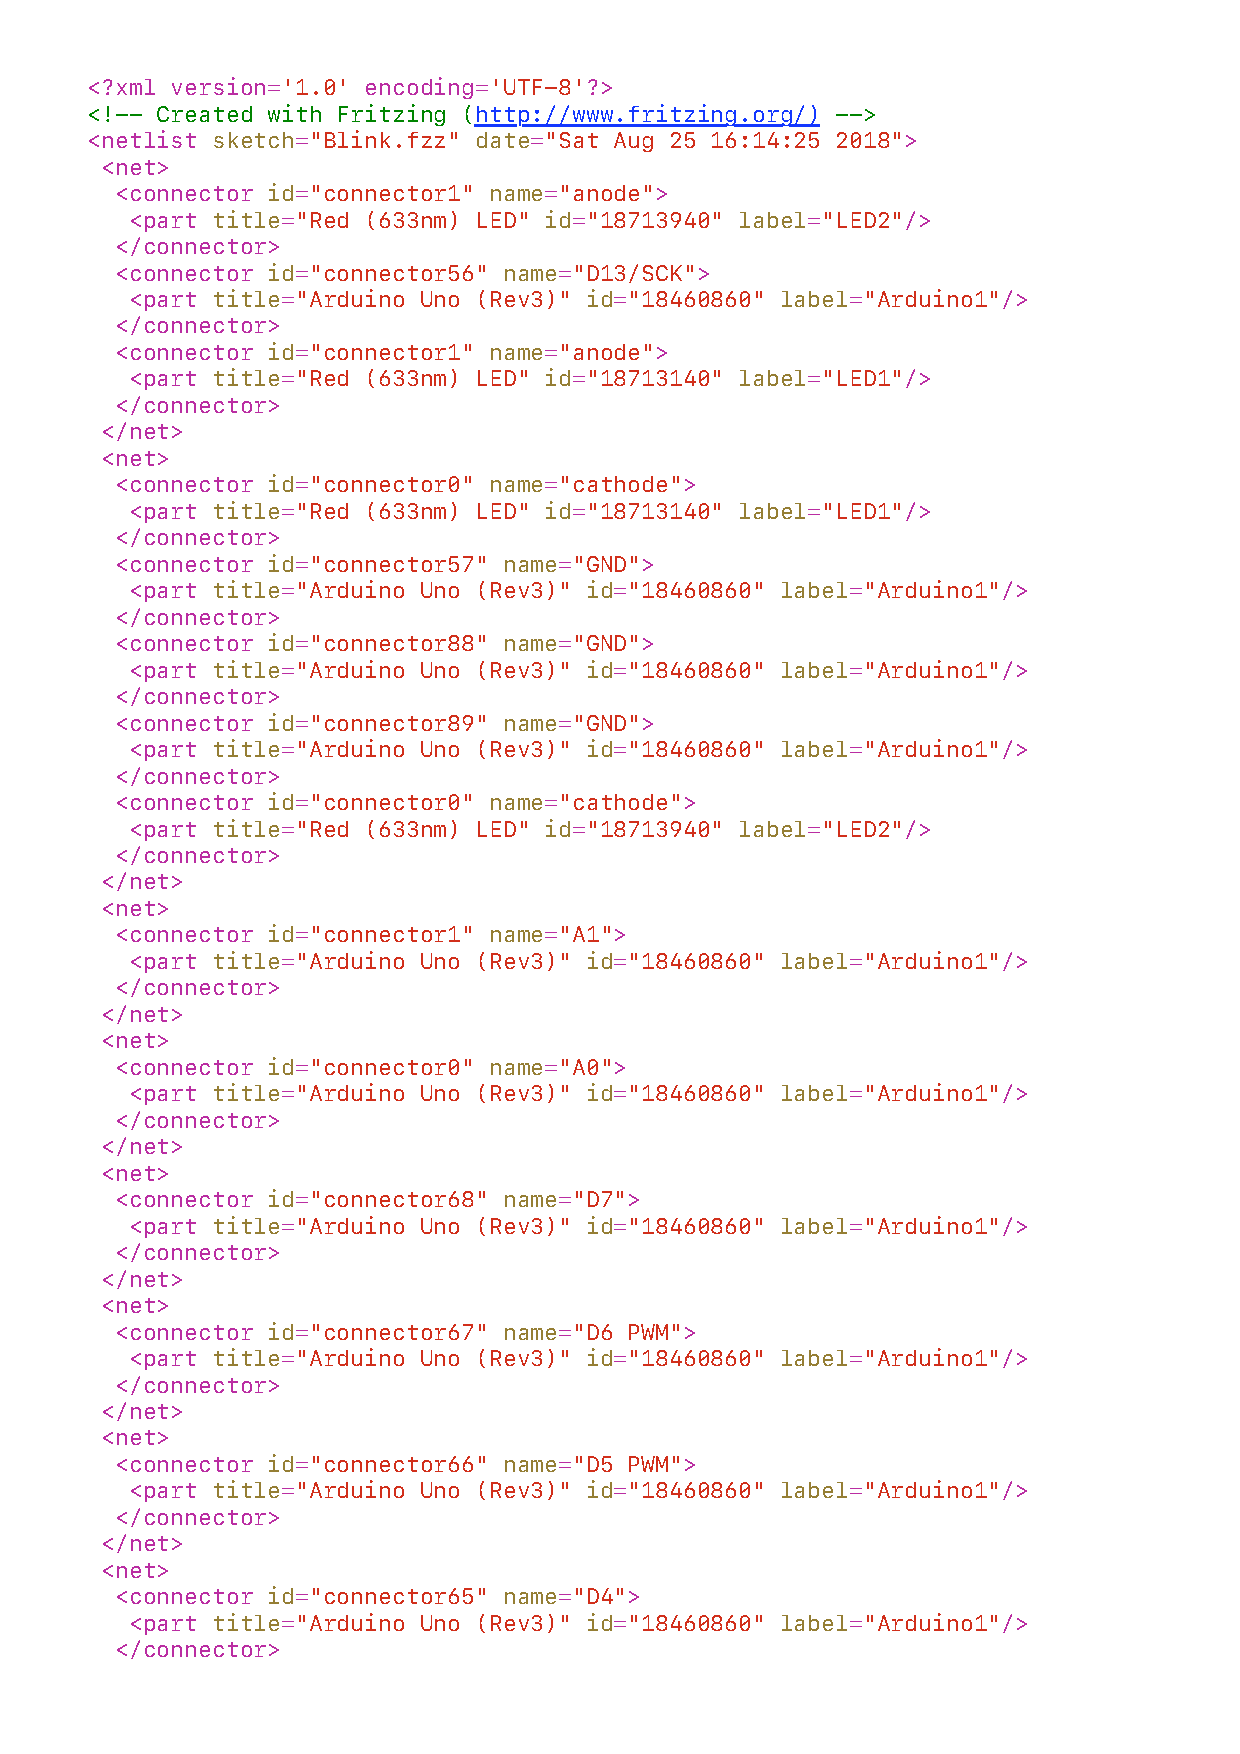
\includepdf[pages=1,scale=0.75, pagecommand=\section{Test Case 2 Netlist}\label{one_pin_netlist}]{graphics/One_Pin.pdf}
\includepdf[pages=2-,scale=0.75, pagecommand={}]{graphics/LCD_netlist.pdf}
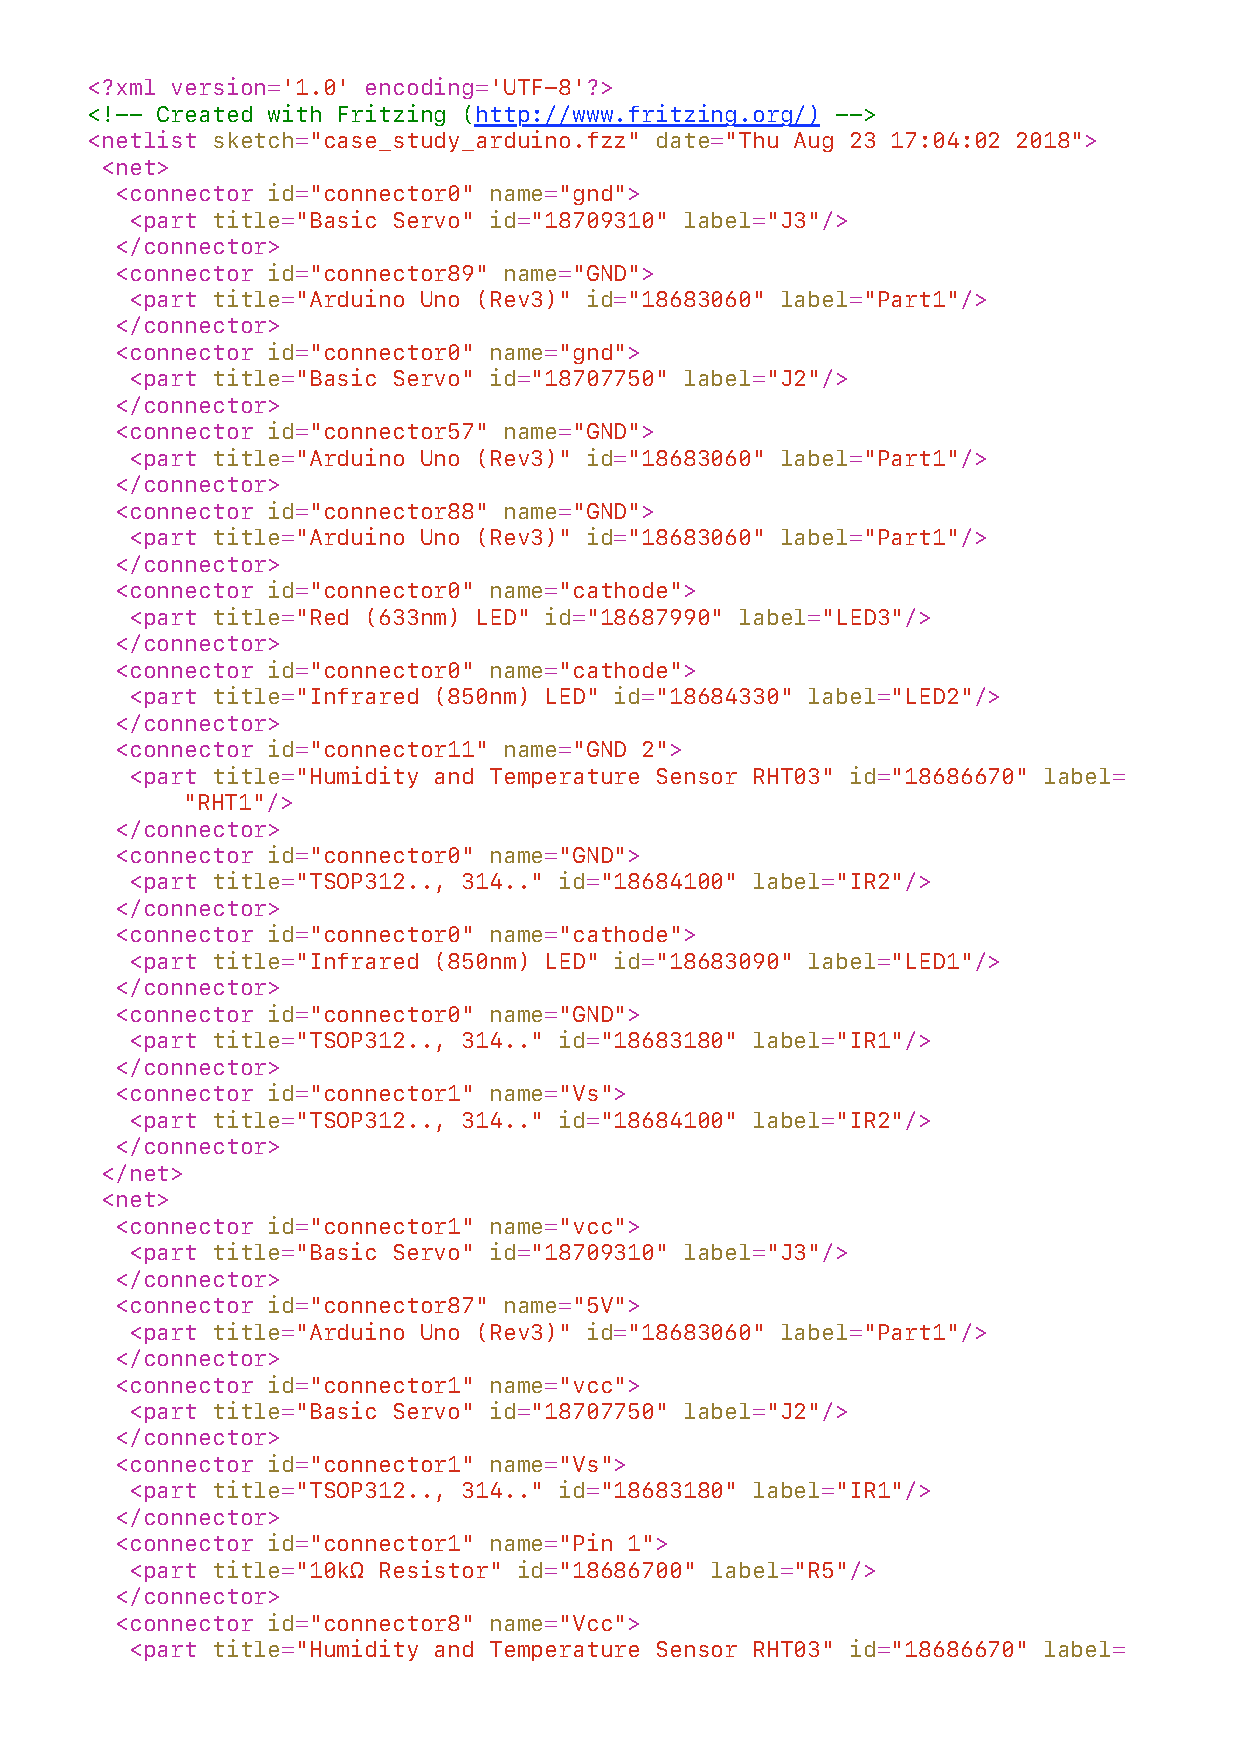
\includepdf[pages=1,scale=0.75, pagecommand=\section{Test Case 3 Netlist}\label{ir_hum_netlist}]{graphics/ir_humidity_sensors_netlist.pdf}
\includepdf[pages=2-,scale=0.75, pagecommand={}]{graphics/ir_humidity_sensors_netlist.pdf}

\chapter{Parallax Source Code Analysis Test Inputs/Outputs}
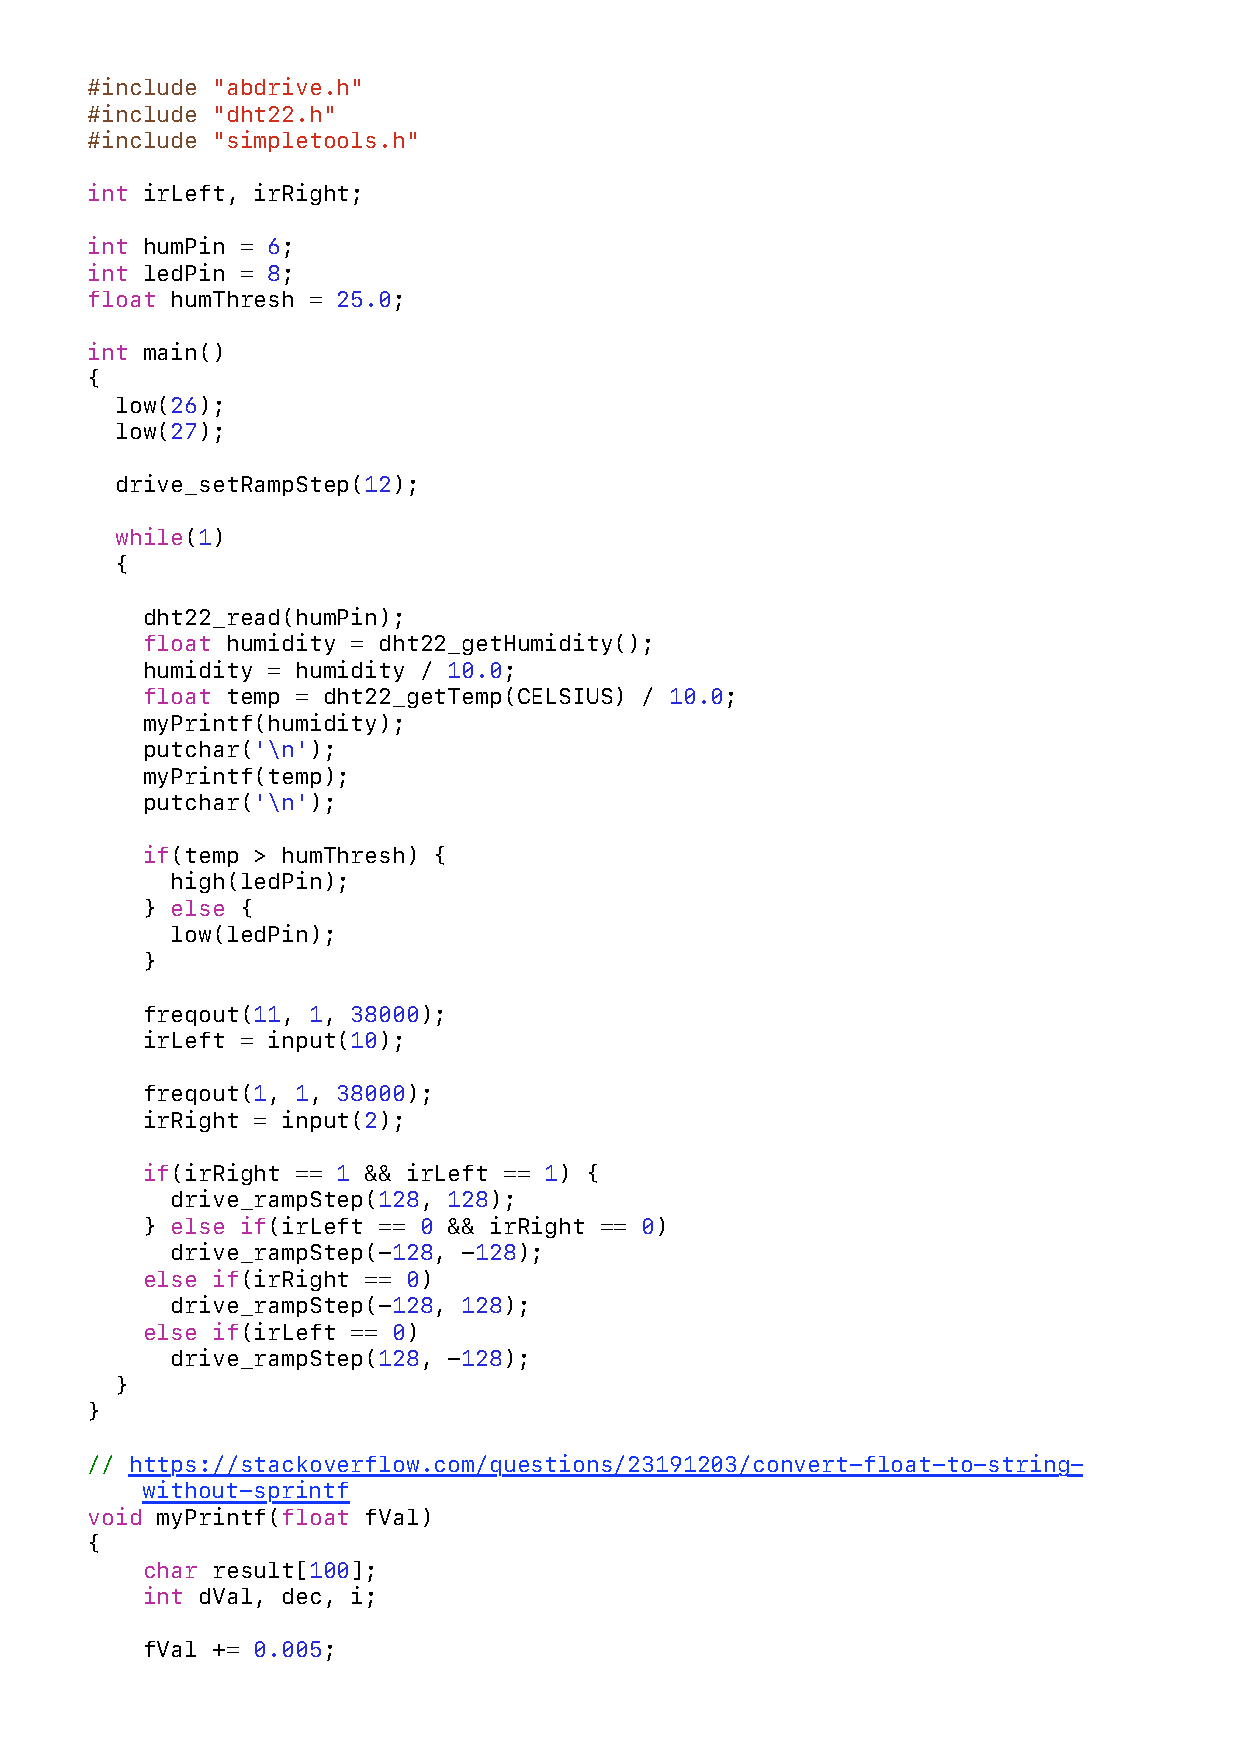
\includepdf[pages=1,scale=0.75, pagecommand=\section{Test Case 1 Parallax Source Input}\label{ir_hum_parallax_in}]{graphics/ir_humidity_sensors_in.pdf}
\includepdf[pages=2-,scale=0.75, pagecommand={}]{graphics/ir_humidity_sensors_in.pdf}
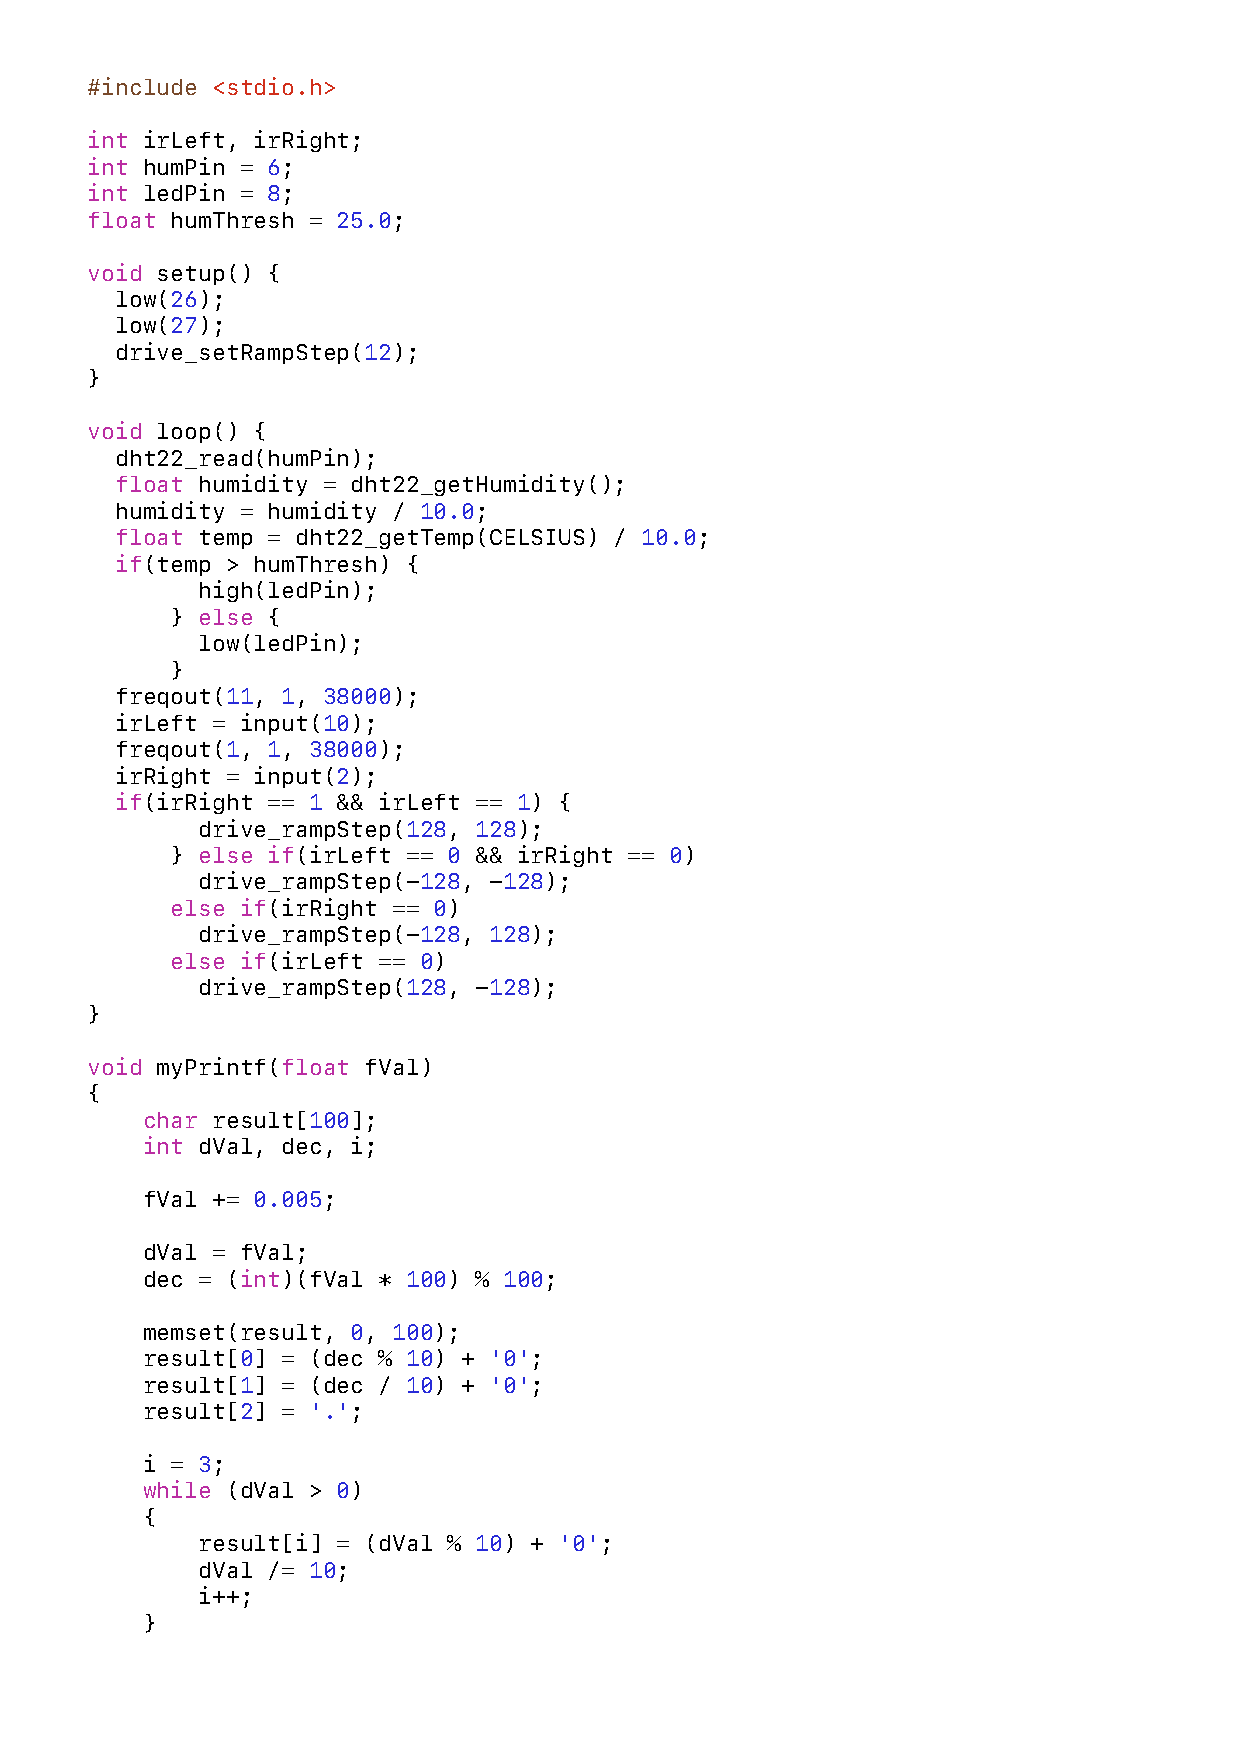
\includepdf[pages=1,scale=0.75, pagecommand=\section{Test Case 1 Parallax Source Output}\label{parallax_tc1_out}]{graphics/parallax_test_case_1_out.pdf}
\includepdf[pages=2-,scale=0.75, pagecommand={}]{graphics/parallax_test_case_1_out.pdf}

\chapter{Case Studies} \label{case_studies}
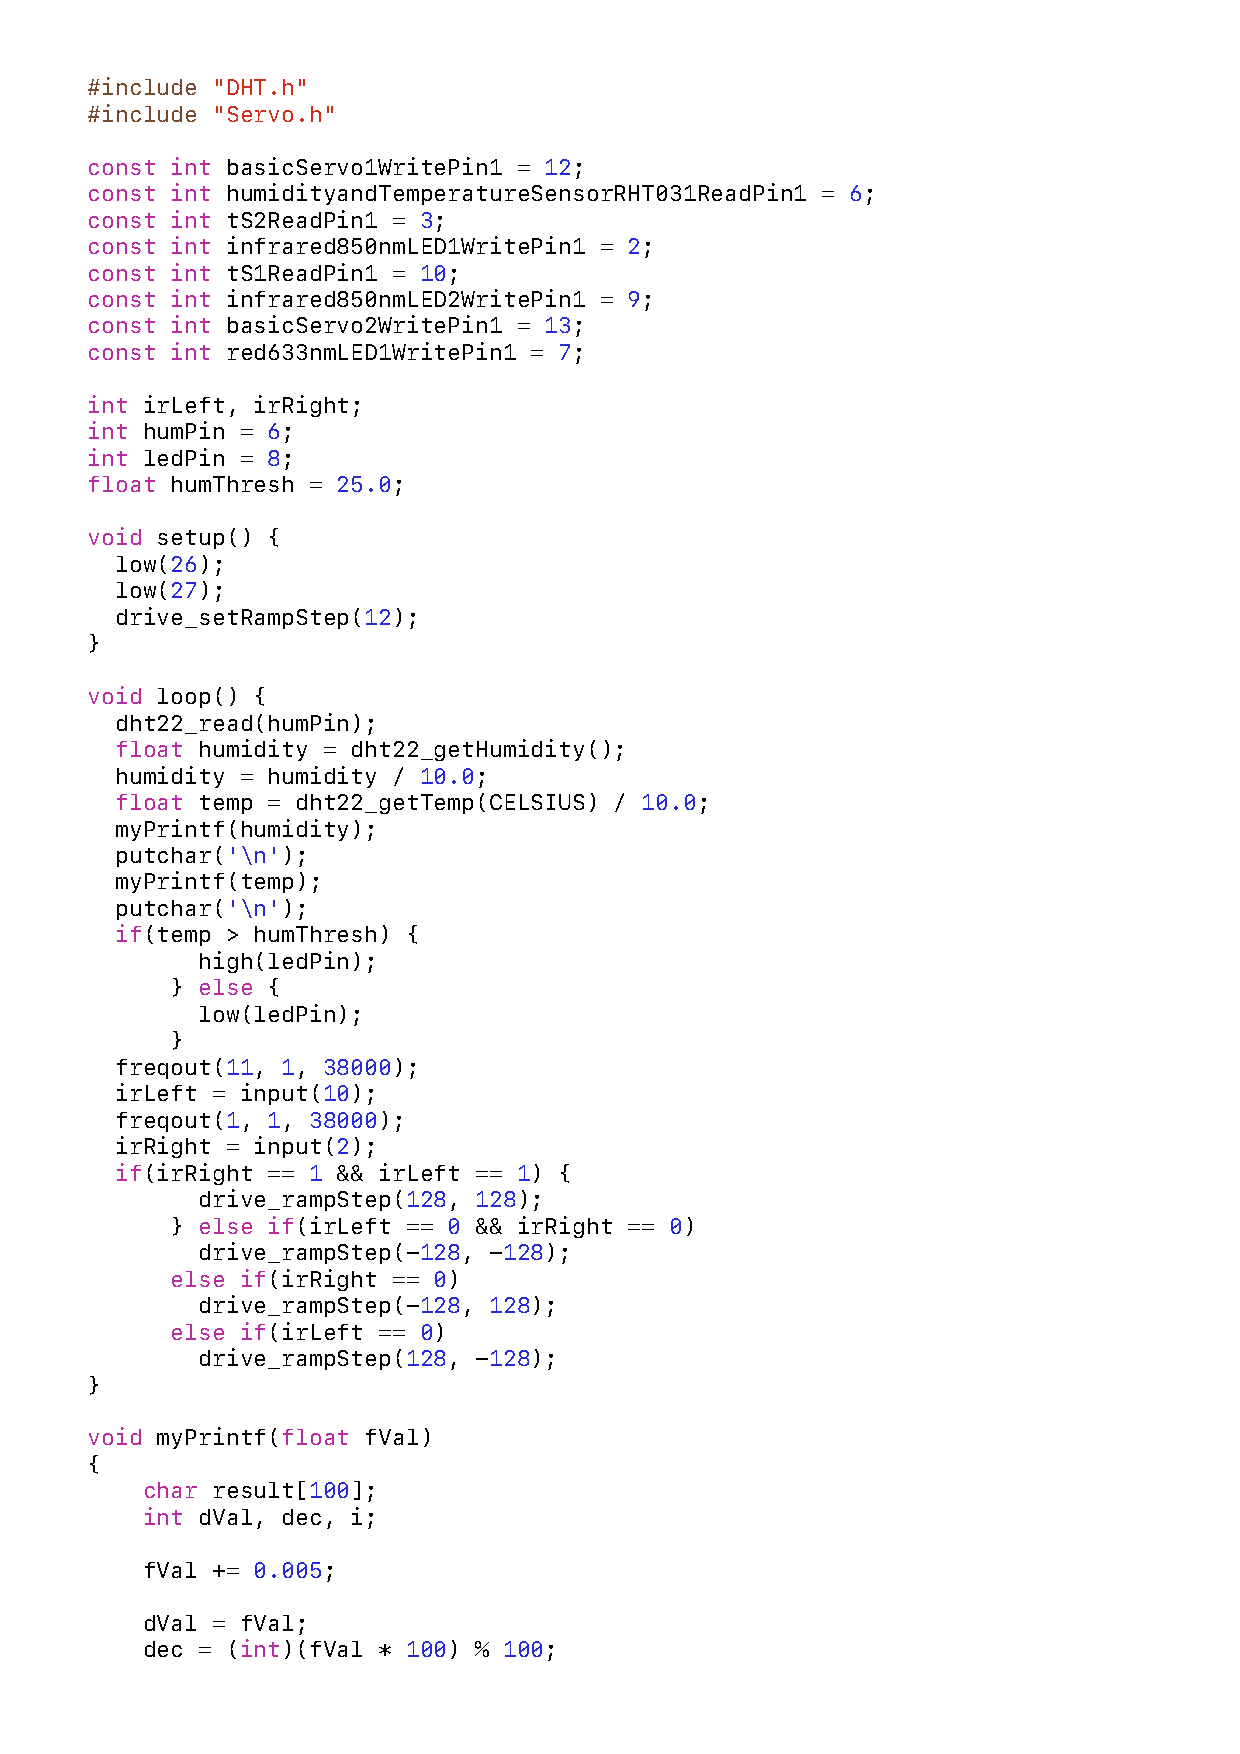
\includepdf[pages=1,scale=0.75, pagecommand=\section{CS-1 Output}\label{cs1_out}]{graphics/ir_humidity_sensors_out.pdf}
\includepdf[pages=2-,scale=0.75, pagecommand={}]{graphics/ir_humidity_sensors_out.pdf}
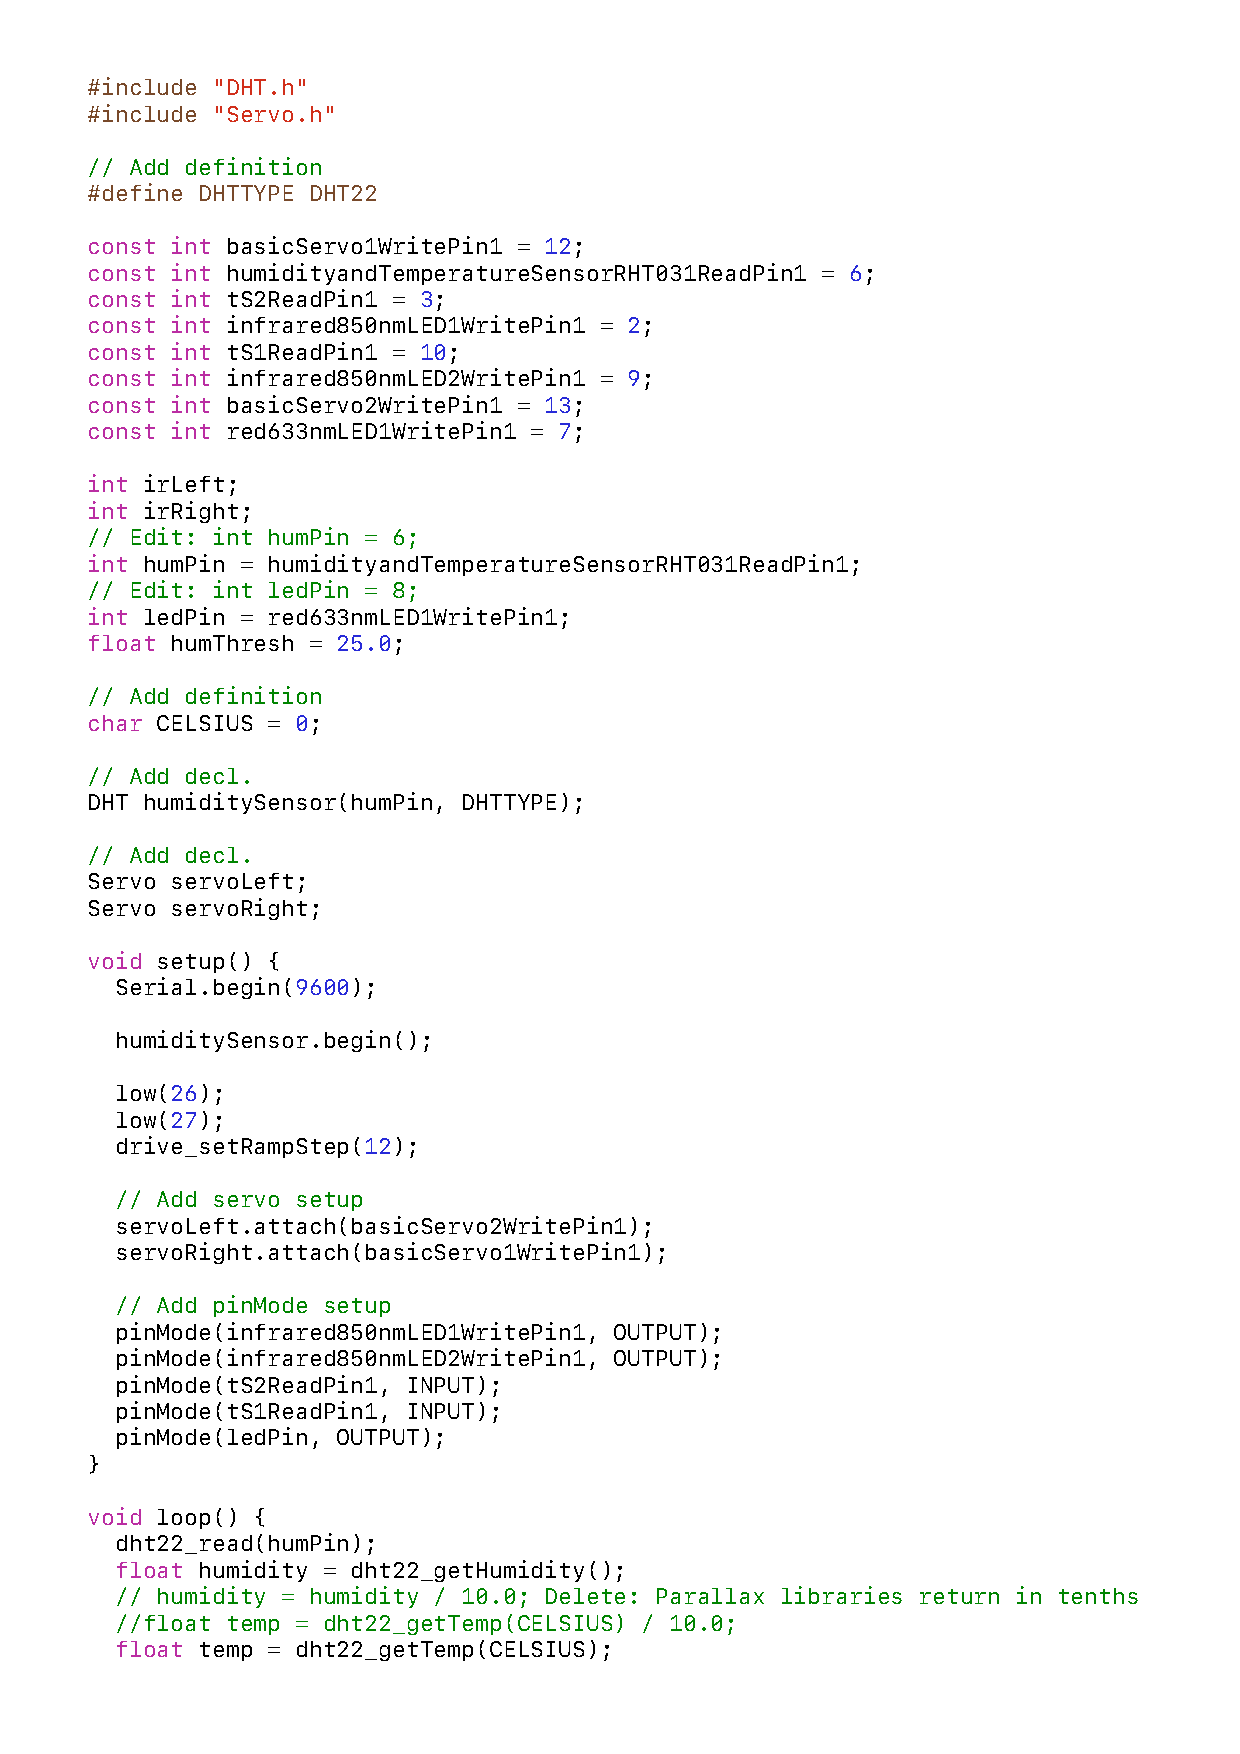
\includepdf[pages=1,scale=0.75, pagecommand=\section{CS-1 Migrated Code}\label{cs1_migrated}]{graphics/ir_humidity_sensors_migrated.pdf}
\includepdf[pages=2-,scale=0.75, pagecommand={}]{graphics/ir_humidity_sensors_migrated.pdf}


\end{appendices}
\end{document}